\pdfoutput=1


\documentclass[11pt]{article}

\usepackage{EMNLP2023}
\usepackage{xspace}

\usepackage{times}
\usepackage{latexsym}
\usepackage{bm}
\usepackage{pifont}
\usepackage{float}       
\usepackage{enumitem}
\usepackage{subfig}                
\usepackage{overpic}               
\usepackage{pgfplots}
\usepackage{soul}

\usepackage[hyphenbreaks]{breakurl}

\usepackage[T1]{fontenc}


\usepackage[utf8]{inputenc}

\usepackage{microtype}

\usepackage{inconsolata}

\usepackage{amsmath}
\usepackage{amssymb}
\usepackage{booktabs}
\usepackage{tikz}
\usepackage{makecell}
\usepackage{graphicx}
\usepackage{multicol}
\usepackage{multirow}



\title{PartialFormer: Modeling Part Instead of Whole}



\author{
Tong Zheng\thanks{\xspace\xspace Equal Contribution.
}~~,
  Bei Li,
  Huiwen Bao,
  Weiqiao Shan,\\
  \textbf{Tong Xiao\thanks{\xspace\xspace Corresponding author.}~~}
  \textbf{and Jingbo Zhu}\\
  School of Computer Science and Engineering, Northeastern University, Shenyang, China\\
  NiuTrans Research, Shenyang, China \\
  {\tt
        \{zhengtong12356, goodbaohuiwen\}@gmail.com, libei\_neu@outlook.com
  }\\
  {\tt
        \{xiaotong,zhujingbo\}@mail.neu.edu.cn
  }
}

\begin{document}
\maketitle
\begin{abstract}
The design choices in Transformer feed-forward neural networks have resulted in significant computational and parameter overhead. In this work, we emphasize the importance of hidden dimension in designing lightweight FFNs, a factor often overlooked in previous architectures. Guided by this principle, we introduce PartialFormer, a parameter-efficient Transformer architecture utilizing multiple smaller FFNs to reduce parameters and computation while maintaining essential hidden dimensions. These smaller FFNs are integrated into a multi-head attention system to enable effective collaboration. We also propose a tailored head scaling strategy to enhance PartialFormer's capabilities. Furthermore, we present a residual-like attention calculation to improve depth scaling within PartialFormer. Extensive experiments on 9 translation tasks and 1 abstractive summarization task validate the effectiveness of our PartialFormer approach. Our code would be available
at: \url{https://github.com/zhengkid/PartialFormer}.
\end{abstract}

\section{Introduction}

The Transformer model~\cite{Vaswani2017transformer} has emerged as a cornerstone in the natural language processing~(NLP) domain, overshadowing convolutional neural networks~\cite{Gehring2017convolutionals2s} and recurrent neural networks~\cite{Sutskever2014sequence2sequence} by virtue of its minimal inductive bias, superior scalability, and proficiency in modeling extended sequences. Nonetheless, its substantial computational and parametric requisites pose significant challenges to its deployment and training, warranting an ongoing trend in the research community toward eliminating redundant parameters and computations~\cite{Dehghani2019UniversalTransformer,Mehta2019DeFINEDF, Lan2020ALBERT, Wu2020Lite, Mehta2021Delight,reid-etal-2021-subformer-exploring,li-etal-2022-ode} in Transformer.

\begin{figure}[ht!]
	\centering
\usetikzlibrary{shapes.geometric}
        \begin{tikzpicture}[]

        \def\nodehsep{1.2em}
        \def\wh{2em}
        \def\ww{1em}
        \def\whsep{0.4em}
        \def\sww{2em}
        \def\swwsep{2.5em}
        \def\reluw{5.5em}
        \def\reluh{1em}
        \def\verytiny{\fontsize{2pt}{5pt}\selectfont}
        
\begin{scope}[xshift=0em]
        {\small
        \node [anchor=north,trapezium, trapezium left angle=120, trapezium right angle=120, minimum width=\ww, minimum height=\wh,fill=orange!30] (w11) at (0, 0) {};

        \node [anchor=south,font=\footnotesize,rectangle, minimum width=\reluw, minimum height=\reluh,fill=blue!20,inner sep=0pt](relu) at ([yshift=\nodehsep]w11.north) {ReLU};

        \node [anchor=south,trapezium, trapezium left angle=60, trapezium right angle=60, minimum width=\ww, minimum height=\wh,fill=orange!30] (w21) at ([yshift=\nodehsep]relu.north) {};
        }

        {\scriptsize
        \node [anchor=north west, inner sep=0em] (s11) at ([xshift=0.5em,yshift=-\whsep]w11.south) {};
        \node [anchor=south west, inner sep=0em] (s12) at ([xshift=0.5em,yshift=\whsep*0.7]w11.north) {};
        \node [anchor=north west, inner sep=0em] (s21) at ([xshift=0.5em,yshift=-\whsep*0.7]w21.south) {};
        \node [anchor=south west, inner sep=0em] (s22) at ([xshift=0.5em,yshift=\whsep]w21.north) {};

        \draw[->] ([yshift=-\nodehsep*0.9]w11.south) -- ([yshift=-0em]w11.south);
        \draw[->] ([yshift=-0em]w11.north) -- ([yshift=-0em]relu.south);
        \draw[->] ([yshift=-0em]relu.north) -- ([yshift=-0em]w21.south);
        }

        \node [anchor=center,rectangle,rounded corners=5pt,draw,dotted,minimum width=\reluw*0.95, minimum height=\wh*4](back) at (relu.center) {};

        \node [anchor=north, font=\footnotesize, inner sep=0em] (l) at ([yshift=-4em]relu.south) {(a) Vanilla};
        \end{scope}

\begin{scope}[xshift=0.85in]
        {\small
        \node [anchor=north,trapezium, trapezium left angle=60, trapezium right angle=60, minimum width=\ww, minimum height=\wh,fill=orange!30] (w11) at (0, 0) {};

        \node [anchor=south,font=\footnotesize,rectangle, minimum width=\ww, minimum height=\reluh,fill=blue!20,inner sep=2pt](relu) at ([yshift=\nodehsep]w11.north) {ReLU};

        \node [anchor=south,trapezium, trapezium left angle=120, trapezium right angle=120, minimum width=\ww, minimum height=\wh,fill=orange!30] (w21) at ([yshift=\nodehsep]relu.north) {};
        }

        {\scriptsize
        \node [anchor=north west, inner sep=0em] (s11) at ([xshift=0.5em,yshift=-\whsep]w11.south) {};
        \node [anchor=south west, inner sep=0em] (s12) at ([xshift=0.5em,yshift=\whsep*0.7]w11.north) {};
        \node [anchor=north west, inner sep=0em] (s21) at ([xshift=0.5em,yshift=-\whsep*0.7]w21.south) {};
        \node [anchor=south west, inner sep=0em] (s22) at ([xshift=0.5em,yshift=\whsep]w21.north) {};

        \draw[->] ([yshift=-\nodehsep*0.9]w11.south) -- ([yshift=-0em]w11.south);
        \draw[->] ([yshift=-0em]w11.north) -- ([yshift=-0em]relu.south);
        \draw[->] ([yshift=-0em]relu.north) -- ([yshift=-0em]w21.south);
        }

        \node [anchor=center,rectangle,rounded corners=5pt,draw,dotted,minimum width=\reluw*0.95, minimum height=\wh*4](back) at (relu.center) {};

        \node [anchor=north, font=\footnotesize, inner sep=0em] (l) at ([yshift=-4em]relu.south) {(b) Lightweight};
        \end{scope}

\begin{scope}[xshift=1.53in]
        {\small
        \node [anchor=north,trapezium, trapezium angle=130, trapezium stretches body=true, minimum width=\sww, minimum height=\wh,fill=orange!30] (w11) at (0, 0) {};
        \node [anchor=center,trapezium, trapezium angle=130, trapezium stretches body=true, minimum width=\sww, minimum height=\wh,fill=orange!30] (w12) at ([xshift=\swwsep]w11.center) {};
        \node [anchor=west, font=\tiny, inner sep=0em,inner sep=0pt] (w13) at ([xshift=\swwsep*0.5]w12.center) {};
        \node [anchor=center,trapezium, trapezium angle=130, trapezium stretches body=true, minimum width=\sww, minimum height=\wh,fill=orange!30] (w14) at ([xshift=\swwsep*0.5]w13.east) {};

        \node [anchor=center, font=\small] (ww11) at (w11.center) {};
        \node [anchor=center, font=\small] (ww12) at (w12.center) {};
        \node [anchor=center, font=\small] (ww14) at (w14.center) {};
        
        \node [anchor=south west,font=\footnotesize,rectangle, minimum width=\reluw*1.45, minimum height=\reluh,fill=blue!20,inner sep=0pt](relu) at ([xshift=-\sww*0.5,yshift=\nodehsep]w11.north) {ReLU};

        \node [anchor=south,trapezium, trapezium angle=60, trapezium stretches body=true, minimum width=\sww, minimum height=\wh,fill=orange!30] (w21) at ([xshift=\sww*0.5,yshift=\nodehsep]relu.north west) {};
        \node [anchor=center,trapezium, trapezium angle=60, trapezium stretches body=true, minimum width=\sww, minimum height=\wh,fill=orange!30] (w22) at ([xshift=\swwsep]w21.center) {};
        \node [anchor=west, inner sep=0em, font=\tiny] (w23) at ([xshift=\swwsep*0.5]w22.center) {};
        \node [anchor=center,trapezium, trapezium angle=60, trapezium stretches body=true, minimum width=\sww, minimum height=\wh,fill=orange!30] (w24) at ([xshift=\swwsep*0.5]w23.east) {};

        \node [anchor=center, font=\tiny] (ww21) at (w21.center) {};
        \node [anchor=center, font=\tiny] (ww22) at (w22.center) {};
        \node [anchor=center, font=\tiny] (ww24) at (w24.center) {};
        }
        {\scriptsize
        \node [anchor=north west, inner sep=0em] (s11) at ([xshift=0.2em]w11.south) {};
        \node [anchor=south west, inner sep=0em] (s12) at ([xshift=0.2em]w11.north) {};
        \node [anchor=north west, inner sep=0em] (s21) at ([xshift=0.2em]w21.south) {};
        \node [anchor=south west, inner sep=0em] (s22) at ([xshift=0.2em]w21.north) {};

        \node [anchor=north west, inner sep=0em] (s11) at ([xshift=0.2em]w12.south) {};
        \node [anchor=south west, inner sep=0em] (s12) at ([xshift=0.2em]w12.north) {};
        \node [anchor=north west, inner sep=0em] (s21) at ([xshift=0.2em]w22.south) {};
        \node [anchor=south west, inner sep=0em] (s22) at ([xshift=0.2em]w22.north) {};

        \node [anchor=north west, inner sep=0em] (s11) at ([xshift=0.2em]w14.south) {};
        \node [anchor=south west, inner sep=0em] (s12) at ([xshift=0.2em]w14.north) {};
        \node [anchor=north west, inner sep=0em] (s21) at ([xshift=0.2em]w24.south) {};
        \node [anchor=south west, inner sep=0em] (s22) at ([xshift=0.2em]w24.north) {};

        \draw[->] ([yshift=-\nodehsep*0.9]w11.south) -- ([yshift=-0em]w11.south);
        \draw[->] ([yshift=-0em]w11.north) -- ([yshift=\nodehsep*1.2]w11.north);
        \draw[->] ([yshift=-\nodehsep*1.2]w21.south) -- ([yshift=-0em]w21.south);

        \draw[->] ([yshift=-\nodehsep*0.9]w12.south) -- ([yshift=-0em]w12.south);
        \draw[->] ([yshift=-0em]w12.north) -- ([yshift=\nodehsep*1.2]w12.north);
        \draw[->] ([yshift=-\nodehsep*1.2]w22.south) -- ([yshift=-0em]w22.south);

        \draw[->] ([yshift=-\nodehsep*0.9]w14.south) -- ([yshift=-0em]w14.south);
        \draw[->] ([yshift=-0em]w14.north) -- ([yshift=\nodehsep*1.2]w14.north);
        \draw[->] ([yshift=-\nodehsep*1.2]w24.south) -- ([yshift=-0em]w24.south);
        }

        \node [anchor=center,rectangle,rounded corners=5pt,draw,dotted,minimum width=\reluw*1.42, minimum height=\wh*4](back) at (relu.center) {};

        \node [anchor=north, font=\footnotesize, inner sep=0em] (l) at ([yshift=-4em]relu.south) {(c) PartialFormer};
        \end{scope}
       
        \end{tikzpicture}
	\caption{Illustration of our idea.}
 \label{fig:merit}
\end{figure} 
While these attempts represent significant strides in enhancing the efficiency of the Transformer architecture, they largely neglect an equally critical component: the Feed-Forward Network (FFN) that constitutes a substantial part of the Transformer's computational and parametric footprint, due to the inherent large feature space and hidden dimension.
Previous studies~\cite{Mehta2021Delight, Wu2020Lite, ge-etal-2022-edgeformer} have simplified FFNs by naively reducing their hidden dimensions, often at the expense of expressive power.
This leads to a question: \textit{Is the current formulation of lightweight FFNs truly optimal?}


To answer this concern, we turn to the insights provided by \citet{geva-etal-2021-transformer}, who depicted FFNs as a collection of key-value memories, where the number of memories is equal to the number of hidden dimensions in FFNs. This finding underscores the significance of hidden dimension in FFNs.
Drawing inspiration from this finding and the successful application of large hidden sizes in FFNs as evidenced by Meta's 4B model~\cite{tran-etal-2021-facebook}\footnote{They 
have shown enlarging the hidden size of FFNs to 16384 delivers significant BLEU improvements.}, 
we hypothesize that an efficient lightweight FFN is not merely about parameter reduction. Rather, it should aim to preserve, or even expand, the hidden dimension while judiciously reducing the number of parameters involved.

The literature on animal cognition provides some clues for designing a lightweight and expressive FFNs. 
Research on animals' behavior has shown that group animals such as insects, fish, and some birds can emerge with some incredible abilities to deal with some complex tasks, though each individual owns poor abilities~\cite{couzin2009collective, conradt2005consensus}. 
This concept resonates with the AI community's ``Swarm Intelligence'' paradigm~\cite{Bonabeau1999SwarmIntelligence}, which emphasizes the power of collective decision-making. This biological prior motivates us to integrate Swarm Intelligence principles into the FFN design process.




To this end, we propose PartialFormer, an innovative approach to Transformer architecture. 
At the heart of PartialFormer lies the novel concept of Partial-Level Gated Feed-Forward Networks (PG-FFN). Conceived as an ensemble of streamlined FFNs operating in concert, each PG-FFN produces lower-dimensional hidden features. Despite their reduced individual dimensions, the aggregated output of these PG-FFNs either matches or surpasses the hidden dimensions of traditional, larger FFNs, as empirically substantiated in Figure \ref{fig:merit}. Moreover, we further equipped PartialFormer with a head scaling strategy tailed for efficiently scaling, and a residual-like attention calculation for stable optimization. These techniques empower PartialFormer to achieve deeper layer stacking or increased width within the same parameter budget.


Our main contributions can be summarized as follows:
\begin{itemize}[itemsep=0pt,topsep=0pt,parsep=0pt]
\item We introduced PG-FFNs, a method that efficiently reduces parameters and computations, and integrated them into the PartialFormer architecture for high performance. Additionally, we introduced an attention calculation method for stable optimization.
    \item We investigated the scalability of PartialFormer and proposed a head scaling strategy tailored for PartialFormer to efficient scaling.
    \item Rigorous empirical tests across 9 machine translation tasks and 1 abstractive summarization task confirm the effectiveness and efficiency of PartialFormer.
\end{itemize}















\section{Preliminary: Transformer}

In this section, we present some prior knowledge about the Transformer.
Transformer block consists of a multi-head self-attention and a feed-forward network. Let  be a  input matrix of  tokens. Each multi-head self-attention component owns  heads. For simplicity, we omit layer normalization and residual connections.

\paragraph{Multi-Head Self-Attention} MHSA aims to model the global dependency among tokens. MHSA computes as follows:

\noindent
where  denote the query, key and value of -th head, which are derived from input with three learnable matrics  as follows: ,  respectively.  is a learnable matrix.  and   denote the attention matrix and representation of -th head, respectively. 



\paragraph{Feed-Forward Network}  Feed-forward network is responsible for improving the expressiveness of the whole representation space by adopting an "expansion-activation-reduction" mapping strategy. It computes as follows:

\noindent where  as learnable matrices and  denotes the hidden dimension in FFN that is usually set to 4.



\begingroup
\usetikzlibrary{shapes.geometric}
\usetikzlibrary{backgrounds}
\definecolor{tiffanyblue}{RGB}{129,216,208}
\definecolor{bangdiblue}{RGB}{0,149,182}
\definecolor{kleinblue}{RGB}{0,47,167}
\definecolor{kabuliblue}{RGB}{26,85,153}
\definecolor{purple}{RGB}{138,43,226}
\begin{figure*}[ht!]
    \centering

      \tikzset{global scale/.style={
    scale=#1,
    every node/.append style={scale=#1}
  }
}


    \begin{tikzpicture}[global scale=0.69]
    \newlength{\moduleintervaly}
    \setlength{\moduleintervaly}{1.8em}    
    \newlength{\moduleintervalx}
    \setlength{\moduleintervalx}{-7em}
    \newlength{\blockintervalx}
    \setlength{\blockintervalx}{30em}
    
    
    
    \tikzstyle{circlenode}=[draw, circle,minimum size=4pt,inner sep=0, fill=red!30];
    
    \tikzstyle{moduleode}=[draw,minimum height=2.5em,minimum width=23em,inner sep=.0em,thick,rounded corners=.2em, font=\small, scale=0.8];
    
    \tikzstyle{layernode}=[draw,minimum height=1.5em,minimum width=5em,inner sep=.0em,thick,rounded corners=.2em, font=\small,fill=yellow!20];
    
    \tikzstyle{attentionnode}=[draw,minimum height=1.5em,minimum width=5em,inner sep=.0em,thick,rounded corners=.2em, font=\small];

    \tikzstyle{querynode}=[draw,minimum height=1.5em,minimum width=2em,inner sep=.0em,thick,rounded corners=.2em, font=\small];

    \tikzstyle{attnmapnode}=[fill=yellow!20,draw,minimum height=2.5em,minimum width=10em,inner sep=.0em,thick,rounded corners=.2em, font=\small];

    \tikzstyle{partialattnmapnode}=[fill=tiffanyblue!40,draw,minimum height=2.5em,minimum width=12em,inner sep=.0em,thick,rounded corners=.2em, font=\small];

    \tikzstyle{partialattnmapnode1}=[fill=red!20,draw,minimum height=2.5em,minimum width=12em,inner sep=.0em,thick,rounded corners=.2em, font=\small];

    \tikzstyle{GRLattnmapnode}=[fill=yellow!20,draw,minimum height=2.5em,minimum width=8em,inner sep=.0em,thick,rounded corners=.2em, font=\small];

    \tikzstyle{StandardFFNnode}=[fill=red!20,draw,minimum height=2.5em,minimum width=23em,inner sep=.0em,thick,rounded corners=.2em, font=\small];

    \tikzstyle{Concatenode}=[draw,minimum height=1.5em,minimum width=5em,inner sep=.0em,thick,rounded corners=.2em, font=\small];

    \tikzstyle{subspace_block}=[fill=yellow!20,draw,minimum height=2.5em,minimum width=8em,inner sep=.0em,thick,rounded corners=.2em, font=\small];

    \tikzstyle{partial_subspace_block}=[fill=red!20,draw,minimum height=2.5em,minimum width=11.0em,inner sep=.0em,thick,rounded corners=.2em, font=\small];

    \tikzstyle{global_partial_subspace_block}=[fill=pink!20,draw,minimum height=2.5em,minimum width=6.5em,inner sep=.0em,thick,rounded corners=.2em, font=\small];

    \tikzstyle{space_block}=[fill=blue!20,draw,minimum height=2.5em,minimum width=23em,inner sep=.0em,thick,rounded corners=.2em, font=\small];
    
    \tikzstyle{Encoder_block}=[draw,minimum height=8.8*\moduleintervaly,minimum width=20em,inner sep=.0em,thick,rounded corners=.2em, font=\small];

    \tikzstyle{GRL_block}=[draw,minimum height=7em,minimum width=8.8*\moduleintervaly,inner sep=.0em,thick,rounded corners=.2em, font=\small];

    \tikzstyle{Partial_Encoder_block}=[draw,minimum height=7.7*\moduleintervaly,minimum width=25em,inner sep=.0em,thick,rounded corners=.2em, font=\small];
    
    \tikzstyle{Graph_structure_learning}=[draw,minimum height=1.6em,minimum width=2.5em,inner sep=.0em,thick,rounded corners=.2em, font=\small,fill=orange!20];

    \tikzstyle{recnode}=[rectangle,rounded corners=5pt,draw,minimum height=1.8em,minimum width=3.5em,inner sep=0em,thick,rounded corners=0.2em,font=\small,fill=orange!20];

    \tikzstyle{recnodewhite}=[rectangle,rounded corners=5pt,minimum height=2.2em,minimum width=3.5em,inner sep=0em,thick,rounded corners=0.2em,font=\small];

    \def\nodehsep{3.5em}
    \def\nodewsep{3.5em}
    
    \begin{scope}[]

    \node[recnode,anchor=south](e1) at (0, 0) {SAN};
    \node[recnode,anchor=south](e2) at ([yshift=\nodehsep]e1.north) {FFN};

    \node[recnode,anchor=west](d1) at ([xshift=\nodewsep]e1.east) {SAN};
    \node[recnode,anchor=south](d3) at ([yshift=\nodehsep]d1.north) {FFN};
    \node[recnode,anchor=south](d2) at ([yshift=\nodehsep*0.25]d1.north) {CAN};

    \begin{pgfonlayer}{background}
\node[anchor=south,minimum height=\nodehsep*2.3,minimum width=4.5em,fill=black!4,rounded corners=5pt,dotted,draw](b1) at ([yshift=-0.5em]e1.south) {};
        \node[anchor=south,minimum height=\nodehsep*2.3,minimum width=4.5em,fill=black!4,rounded corners=5pt,dotted,draw](b2) at ([yshift=-0.5em]d1.south) {};
    \end{pgfonlayer}

   \draw[->,thick] ([yshift=-1.0em]e1.south) -- (e1.south);
   \draw[->,thick] (e1.north) -- (e2.south);

   \draw[->,thick] ([yshift=-1.0em]d1.south) -- (d1.south);
   \draw[->,thick] (d1.north) -- (d2.south);
   \draw[->,thick] (d2.north) -- (d3.south);
   \draw[->,thick] (d3.north) -- ([yshift=1.0em]d3.north);

   \draw[->,thick] (e2.north) -- ([yshift=1em]e2.north) -- ([xshift=\nodewsep*1.05,yshift=1em]e2.north) -- ([xshift=-\nodewsep*0.48]d2.west) -- (d2.west);

    \node[anchor=south west](n) at ([xshift=-0.4em]b1.north west) {};
    \node[anchor=south west](m) at ([xshift=-0.4em]b2.north west) {};
    
    \node[anchor=south,font=\Large](l1) at ([xshift=3.5em,yshift=-3em]e1.south) {(a) Transformer};
    \node[anchor=west,font=\Large](l2) at ([xshift=0.8in]l1.east) {(b) PartialFormer};
    \node[anchor=west,font=\Large](l3) at ([xshift=1.2in]l2.east) {(c) PartialFormer Self-AFFN Block};
    
    \end{scope}

    \begin{scope}[xshift=2.2in,yshift=0.0in]

    \node[recnodewhite,anchor=south](e1) at (0, 0) {};
    \node[recnodewhite,anchor=south](e2) at ([yshift=\nodehsep]e1.north) {};

    \node[recnode,anchor=south,minimum width=5em](e3) at ([yshift=\nodehsep*0.2]e1.north) {Self-AFFN};

    \node[recnode,anchor=west,minimum width=5em,dashed,draw,very thick,fill=orange!40](d1) at ([xshift=\nodewsep]e1.east) {Self-AFFN};
    \node[recnodewhite,anchor=south](d3) at ([yshift=\nodehsep]d1.north) {};
    \node[recnode,anchor=south,minimum width=5em](d2) at ([yshift=\nodehsep*0.2]d1.north) {Cross-AFFN};

    \begin{pgfonlayer}{background}
\node[anchor=south,minimum height=\nodehsep*0.77,minimum width=6em,fill=black!4,rounded corners=5pt,dotted,draw](b1) at ([yshift=-0.5em]e3.south) {};
        \node[anchor=south,minimum height=\nodehsep*1.6,minimum width=6em,fill=black!4,rounded corners=5pt,dotted,draw](b2) at ([yshift=-0.5em]d1.south) {};
\end{pgfonlayer}

   \draw[->,thick] (e1.north) -- (e3.south);
   \draw[->,thick] ([yshift=-1.0em]d1.south) -- (d1.south);
   \draw[->,thick] (d1.north) -- (d2.south);
   \draw[->,thick] (d2.north) -- (d3.south);


   \draw[->,thick] (e3.north) -- ([yshift=1em]e3.north) -- ([xshift=\nodewsep*1.16,yshift=1em]e3.north) -- ([xshift=-\nodewsep*0.36]d2.west) -- (d2.west);

    \node[anchor=south west](n) at ([xshift=-0.4em]b1.north west) {};
    \node[anchor=south west](m) at ([xshift=-0.4em]b2.north west) {};







   \draw[->,very thick,dashed] ([xshift=0.8em, yshift=-0.5em]d1.south east) -- ([xshift=2.5em, yshift=-0.5em]d1.south east);
  \draw[->,very thick,dashed] ([xshift=0.8em, yshift=0.5em]d1.north east) -- ([xshift=2.3em, yshift=\nodehsep*2.8]d1.north east);
  


    \end{scope}
    

    \begin{scope}[xshift=6.15in,yshift=-0.1in]

    \node[font=\small] (block_input) at (0, 0) {\textbf{}};
    
    \node[align=center, font=\small] (Encoder) at ([yshift=3*\moduleintervaly]block_input.center) {};

    \begin{pgfonlayer}{background}
        \node[Partial_Encoder_block, align=center, font=\small] (Encoder_b) at ([yshift=2.1em]Encoder.center) {};
    \end{pgfonlayer}
    
    \node[align=center, font=\small] (Subspace_1) at ([xshift=-5em, yshift=-1.5*\moduleintervaly]Encoder.center) {};

    \node[partial_subspace_block,align=center, font=\small] (Subspace_11) at ([xshift=-6.50em, yshift=-1.5*\moduleintervaly]Encoder.center) {};


\node[querynode,align=center, font=\small] (Subspace_1_g) at ([xshift=-5.6em]Subspace_1.center) {};
    
    \node[querynode,align=center, font=\small] (Subspace_1_q) at ([xshift=-2.9em]Subspace_1.center) {};

    \node[querynode,align=center, font=\small] (Subspace_1_k) at ([xshift=-0.2em]Subspace_1.center) {};

    \node[querynode,align=center, font=\small] (Subspace_1_v) at ([xshift=2.5em]Subspace_1.center) {};


    \node[align=center, font=\small] (Subspace_8) at ([xshift=5em, yshift=-1.5*\moduleintervaly]Encoder.center) {};

    \node[partial_subspace_block,align=center, font=\small] (Subspace_88) at ([xshift=6.50em, yshift=-1.5*\moduleintervaly]Encoder.center) {};

    \node[querynode,align=center, font=\small] (Subspace_8_q) at ([xshift=-2.5em]Subspace_8.center) {};

    \node[querynode,align=center, font=\small] (Subspace_8_k) at ([xshift=0.2em]Subspace_8.center) {};

    \node[querynode,align=center, font=\small] (Subspace_8_v) at ([xshift=2.9em]Subspace_8.center) {};
    \node[querynode,align=center, font=\small] (Subspace_8_g) at ([xshift=5.6em]Subspace_8.center) {};

    
    
    \node[align=center,thick, scale=2] (omit) at ([xshift=5em]Subspace_1.center) {...};

    \node[align=center,thick, scale=2] (omit1) at ([yshift=2*\moduleintervaly]omit.center) {...};
    \node[align=center,thick, scale=2] (omit2) at ([yshift=1.6*\moduleintervaly]omit1.center) {...};


    \draw[->] (block_input) -- (Subspace_11);
    \draw[->] (block_input) -- (Subspace_88);
    \draw[->] (block_input) -- (omit);
    
   \node[partialattnmapnode1,align=center, font=\footnotesize, scale=0.8] (Subspace_8_A) at ([xshift=0.9em,yshift=2*\moduleintervaly]Subspace_8.center) {};

   \draw[->] (Subspace_8_k) -- (Subspace_8_A);
   \draw[->] (Subspace_8_q) -- (Subspace_8_A);
   \draw[->] (Subspace_8_v) -- (Subspace_8_A);

   \node[partialattnmapnode1,align=center, font=\footnotesize, scale=0.8] (Subspace_1_A) at ([ xshift=-0.9em,yshift=2*\moduleintervaly]Subspace_1.center) {};

   \draw[->] (Subspace_1_k) -- (Subspace_1_A);
   \draw[->] (Subspace_1_q) -- (Subspace_1_A);
   \draw[->] (Subspace_1_v) -- (Subspace_1_A);



   \node[partialattnmapnode,align=center, font=\footnotesize, scale=0.8] (Subspace_8_EA) at ([ xshift=0.9em,yshift=3.6*\moduleintervaly]Subspace_8.center) {};

   \node[partialattnmapnode,align=center, font=\footnotesize, scale=0.8] (Subspace_1_EA) at ([xshift=-0.9em, yshift=3.6*\moduleintervaly]Subspace_1.center) {};

   
   \draw[->] (Subspace_8_A) -- (Subspace_8_EA);
   \draw[->] (Subspace_1_A) -- (Subspace_1_EA);







    \draw[->] ([xshift=-0.5em, yshift=0.75em]Subspace_1_g.center) |- (Subspace_1_EA);
    \draw[->] ([xshift=0.5em, yshift=0.75em]Subspace_8_g.center) |- (Subspace_8_EA);



    \node[StandardFFNnode,align=center, font=\footnotesize, scale=0.8] (Final_Agg) at ([xshift=-5em, yshift=5.2*\moduleintervaly]Subspace_8.center) {};



\draw[->] (Subspace_8_EA) -- (Final_Agg);
   \draw[->] (Subspace_1_EA) -- (Final_Agg);

    \end{scope}


  

    
    \end{tikzpicture}
    
    
    
    \caption{(a) Architecture of Transformer. (b) Architecture of PartialFormer. (c) Details of Self-AFFN Block. All architecture are based on pre-normalization strategy. We omit the layer normalization operation, residual connection, softmax operation and scale coefficient for simplicity.     }
    \label{fig:architecture}
\end{figure*}
\endgroup 
\section{PartialFormer}
\subsection{Overall Architecture}
Figure \ref{fig:architecture} illustrates the overall architecture of PartialFormer, encompassing both an encoder and a decoder. Although the foundational structure adheres to the design of the vanilla Transformer~\cite{Vaswani2017transformer}, there are some notable modifications.

\paragraph{Encoder.}
Different from vanilla Transformer, each encoder layer in PartialFormer consists of a unified sub-layer that integrates the PG-FFNs into the multi-head self-attention mechanism.

\paragraph{Decoder.}
Each decoder layer is composed of two types of sub-layers, both of which integrate the multi-head attention mechanism with PG-FFNs. The sub-layers differ based on the type of multi-head attention mechanisms employed, specifically whether it's a decoder self-attention or an encoder-decoder cross-attention mechanism. 
Notably, this design is inspired by previous studies~\cite{Lu-etal-2020-Macaron, Gulati-etal-2020-conformer}, but it differs in that we employ small FFNs, known as PG-FFNs, within each attention head of both the self-attention and cross-attention modules. To reduce computation, we halved the hidden dimension of PG-FFNs. Further decoder comparisons are in Appendix \ref{sec_compare_decoder}.


\subsection{Information Flow in Unified Sub-Layer}
We take the Encoder as an instance. Each unified sub-layer first computes the multiple attention scores via Eq. (\ref{eq:pgffn_score_calculation}), then obtains the multiple head features  via Eq. (\ref{eq:agg}), which is the same as vanilla Transformer. Then, using multiple small FFNs, it processes these head features and ultimately combines the representations via a fusion function according to Eq. (\ref{eq:pgff_fusion}).  That is to say, the PG-FFN is encapsulated into the multihead-attention mechanism.
\noindent

\noindent 

\subsection{Partial-Level Gated FFN}

\paragraph{Intuition}





Previous studies~\cite{Wu2020Lite, Mehta2021Delight, ge-etal-2022-edgeformer} commonly reduced the parameters in feed-forward networks by decreasing the hidden dimension (e.g., 2048 to 256). In contrast, we tackle this issue through a matrix factorization approach. Our key idea involves utilizing a collection of small FFNs to model smaller input features expecting these smaller FFNs to emerge better performance while consuming fewer parameters, akin to ``Swarm Intelligence''

Assume a FFN with mappings of 1024->4096->1024, which consumes around 8.4 million parameters. By decomposing this into 8 smaller FFNs with mappings of 128->512->128, we can retain the same hidden dimension, such as 8 * 512, while using only 1.05 million parameters. This approach significantly reduces parameters while maintaining the crucial hidden dimension, as emphasized in \citet{geva-etal-2021-transformer, tran-etal-2021-facebook}.


Additionally, we have observed that the Transformer architecture inherently consists of multiple smaller subspaces, namely ``heads'' within the multi-head attention (MHA) mechanism. These heads act as sub-components of the original inputs and retain substantial information from the original data. Besides, the fusion mechanism in MHA enables the consolidation of the capabilities of multiple FFNs. As a result, PG-FFNs should naturally be constructed based on the MHA mechanism.


\paragraph{Calculation of PG-FFNs}
While group transformation operations could be used to instantiate our idea, they are not optimal on GPUs due to their low I/O efficiency~\cite{Ningning2018shufflenetv2}, causing significant inference latency. To address this, we propose sharing parameters across each FFN within different heads, thereby eliminating the need for group transformation operations.


However, directly sharing weights may result in homogeneous representations across different heads, which may potentially hinder the performance~\cite{li-etal-2018-multi-head}.  To mitigate this, we further introduce a head-specific gated mechanism. The core idea is to use a set of diverse masks to filter the information of different heads so that the head representation will be more diverse. Formally, given a set of smaller features  and diverse masks , the Eq. (\ref{eq:pgffn}) can rewritten as: 
\noindent

\noindent
\noindent where   is the same as Eq. (\ref{eq:ffn}). 


\paragraph{Generating } 
In our preliminary experiments, we observed significant diversity in the features generated by different parameters from sub-layer inputs, e.g., . Motivated by this finding, we generate diverse masks in the following manner:



\noindent
where  is a learnable matrix and  denotes the activation function, e.g., ReLU, Sigmoid and Tanh. We compare them in Table \ref{tab:layer_ablation_en_de}.


\subsection{Efficient Scaling Strategy}
\label{subsec:scale_mechanism}



Though PG-FFN offers the advantage of reducing lots of parameters when applied directly to the transformer, it also leads to marginal performance degradation~(see Table \ref{tab:result_PG_FFNs_only}). Thus, a crucial aspect of this study is to determine how to effectively utilize the spared parameters. In this work, we adopt a hybrid scaling strategy, which has been validated in computer vision, e.g., EfficientNet~\cite{tan2019efficientnet}. Note that our approach differs from EfficientNet, as we incorporate a combination of head scaling and depth scaling into our methodology.




\subsubsection{Enabling Efficient Depth Scaling for PartialFormer}
\citet{Dong2021PureAttention, Wang2022AntiOversmoothing} have shown that the original location of FFNs plays an essential role in optimizing transformers, e.g., alleviating \textit{Token Uniformity}. Therefore, it's vital to consider the impact of altering the FFN placement. Densely residual connections are effective but typically implemented either at the feature level (e.g., DLCL~\cite{wang-etal-2019-learning-deep}) or integrated into the network structure (e.g., Realformer~\cite{he-etal-2021-realformer}), which are not flexible.

To this end, we design a new variant of the residual connection integrated into the attention calculation, while also decoupling from the network architecture. Specifically, the calculation of attention maps consists of two parts: 1) , the global part, and 2) , the local part. The calculation of  remains the same as in the vanilla Transformer, while  is computed once by using the original embedding as input through Eq. (\ref{eq:score_calculation}).
Inspired by \citet{he-etal-2021-realformer}, to efficiently fuse these components, we add them together and apply a Softmax function, as shown in Eq. (\ref{eq:pgffn_score_calculation}).




In addition to the benefit of efficient depth scaling~(See Appendix \ref{sec:analysis_tu}), this approach provides remarkable flexibility in combining different attention mechanisms, specifically tailored to address specific conditions. For instance, it allows for the utilization of local attention to calculate  when dealing with small datasets~(see Appendix \ref{sec:partial_different_A_G}).




\begin{table*}[t!]
    \centering
    \renewcommand{\arraystretch}{1}
\centering
\small

\setlength{\tabcolsep}{1.5pt}
\resizebox{0.86\linewidth}{!}{\begin{tabular}{clrrrrrccc}
\toprule

\bf Type &\bf Model & -&  &   &  & \bf Param & \bf BLEU & \bf COMET-22 & \bf sBLEU  \\
\midrule
\multirow{4}{*}{\bf \makecell{Multi-Branch \\ Architecture }} & Weighted Transformer~\cite{Ahmed2017WeightedTransformer} & 6-6 & 1024 &-&- & 211M & 28.90 & - & -\\
&Multi-Unit Transformer~\cite{yan-etal-2020-multi} & 6-6 & - & -  &  - & 130M & 29.30 & - & - \\
&MAT~\cite{Fan2020MultibranchAT} & 6-6 & - & - & -  & 206M & 29.90 & - & - \\
&Multi-Path Transformer~\cite{lin-etal-2022-multi-path} & 6-6 & - & - & -  & 193M & 29.68 & - & - \\
\midrule
\multirow{2}{*}{\bf \makecell{Lightweight \\ Architecture}}&Evolved Transformer~\cite{So2019EvolvedTransformer} & - & - & -&-  &64M & 28.20 & - & -\\
&Delight~\cite{Mehta2021Delight} & - & 640 &- &- &54M & 28.00 & - & -\\
\midrule
\multirow{5}{*}{\bf \makecell{Weight Sharing}}&Universal Transformer~\cite{Dehghani2019UniversalTransformer} & - & 1024 & -&-  &65M & 28.90 & - & - \\
&SubFormer~\cite{reid-etal-2021-subformer-exploring} & - & - & - &- &63M & 28.50 & - & -\\
&SubFormer-big~\cite{reid-etal-2021-subformer-exploring} & - & - & -&- &197M & 29.30 & - & - \\
&ODE Transformer (RK4)~\cite{li-etal-2022-ode} & 6-6 & 512 & - & -  & 62M & 29.03 & - & 27.9 \\
&ODE Transformer (RK2, Learn.)~\cite{li-etal-2022-ode} & 24-6 & 512 & - & -  & 118M & 30.29 & - & 29.2 \\
\midrule
\multirow{3}{*}{\bf \makecell{Other \\ Comparisons}} 
&RealFormer~\cite{he-etal-2021-realformer} & 18-18 & 512 & 64 & 8  & 151M & 29.35 & - & -\\
&DMAN~\cite{fan-etal-2021-mask} & 6-6 & 512 & 64 & 8  & 63M & 29.10 & - & - \\
&Mega-Softmax~\cite{Ma2022mega} & 6-6 & 512 & - & 1  & 67M & 29.01 & - & 28.0\\
\midrule
\multirow{10}{*}{\bf Our System} 
&Transformer & 24-6 & 512 & 64 & 8-8 & 118M & 29.05 & 83.60 & 27.9 \\
&PartialFormer (w/o Head Scaling) &24-6 & 512 & 64 & 8-8 & 66M &  28.86 & 83.35 & 27.7
\\
&PartialFormer &24-6 & 512 & 64 & 24-16 & 115M &  30.09 & 84.17 & 29.0\\
\cmidrule(r){2-10}
&Transformer & 6-6 & 512 & 64 & 8-8 & 62M & 27.43 & 82.19 & 26.4 \\
& PartialFormer (w/o Head Scaling) &	6-6	& 512	& 64	& 8-8	& 42M &	27.15	& 81.75	& 26.1 \\
& PartialFormer &	6-6	& 512	& 64	& 24-16 & 63M &	28.60 &	83.21 & 27.5 \\
\cmidrule(r){2-10}
&Transformer & 24-6 & 360 & 45 & 8-8  & 62M & 28.00 & 82.72 & 27.0 \\
&PartialFormer (w/o Head Scaling) &24-6 & 360 & 45 & 8-8 & 36M &  27.88& 82.49 & 26.8\\
&PartialFormer &24-6 & 360 & 45 & 24-16 & 61M &  29.23 & 83.74 & 28.1\\
&PartialFormer &24-6 & 360 & 45 & 30-16 & 68M &  29.56 & 83.94 & 28.4 \\

\bottomrule
\end{tabular}}
    \caption{Results on the WMT'14 En-De task. All method scores are sourced from the original paper. For a fair comparison, we also re-implemented some powerful models, and the results are provided in the appendix.}
    \label{tab:result_main_en_de}
\end{table*}







\subsubsection{Head Scaling: A  Tailored Scaling for PartialFormer}

As aforementioned, PartialFormer is guided by ``swarm intelligence'' and operates with small subspaces. Expanding the number and size of these subspaces intuitively augments PartialFormer's capabilities. In response to this insight, we introduced a head-scaling strategy tailored specifically for PartialFormer, involving the direct addition of more heads and the expansion of their width, effectively bolstering its overall performance.


To achieve this objective, we decouple the relationship between the number of heads and the embedding size, specifically . This approach shares similarities with methods discussed in Bhojanapalli et al. (2020). However, it differs in its two-step process, which draws inspiration from the inherent redundancy observed in attention maps as discussed in \citet{michel2019sixteen, clark-etal-2019-bert, voita-etal-2019-analyzing, nguyen2022improving}. Given values for , , and , we first create intermediate values for  and , and then we expand the attention maps to the desired number of heads using a robust MLP network. In the case of , we generate them directly. This approach allows for the inclusion of more heads in PartialFormer while maintaining the same parameter budget.

We demonstrate that this scaling strategy is naturally well-suited for PartialFormer (see Section \ref{sec:analysis_scaling_strategy_partialformer}). Furthermore, it can also be regarded as a variation of width scaling, offering two significant advantages: 1) enabling flexible imbalanced computation distribution in encoder-decoder architecture, and 2) preventing an excessive distribution of parameters in the embedding and output layers.





\section{Experimental Setups}
We assess PartialFormer's performance across both machine translation and abstractive summarization tasks\footnote{We tested PartialFormer's performance in language modeling, with results in the Appendix.}. More details are given in Appendix \ref{sec:detailed_settup}.

\paragraph{Dataset.} For machine transaltion task, we select 9 datasets involving WMT'14 English-German (En-De), WMT'14 English-French (En-Fr), WMT'16 English-Romanian (En-Ro), and six translation tasks from WMT'17 benchmark. We preprocess the raw data following the standard strategy. For the abstractive summarization task, we utilized the widely-used CNN-DailyMail dataset. We followed the same preprocessing approach as described in ~\citet{ott-etal-2019-fairseq}. We applied joint byte pair encoding (BPE)~\cite{sennrich-etal-2016-neural} with sizes of 32K for all the tasks except the En-Ro task (20K), CNN-DailyMail~(30K). 
 

\paragraph{Training \& Evaluation.}

We train models on GeForce RTX 3090 cards via Fairseq~\cite{ott-etal-2019-fairseq} toolkit primarily following the training strategy in \citet{wang-etal-2019-learning-deep}. For machine translation evaluation, we utilized \textit{multi-BLEU}~\cite{papineni-etal-2002-bleu}, COMET-22~\cite{rei-etal-2022-comet} and sacreBLEU~\cite{post-2018-call} scores. Following \citet{wang-etal-2019-learning-deep}, beam sizes were 4, 4, and 5 for En-De, En-Fr, and En-Ro tasks respectively. \textit{Length\_penalty} of 0.6, 0.8, and 1.3 were applied to En-De, En-Fr, and En-Ro tasks respectively. For the WMT'17 benchmark, beam size and \textit{Length\_penalty} were set to 4 and 1, respectively. We used an ensemble of last 10 checkpoints. For abstractive summarization, we set beam size, \textit{Length\_penalty}, minimum length and maximum length to 4, 2.0, 55 and 140, respectively. The evaluation metric was F1-Rouge~\cite{lin-2004-rouge}(Rouge-1,
Rouge-2 and Rouge-L).




\section{Experiments}
\subsection{Machine Translation}
Table \ref{tab:result_main_en_de} presents the results for the WMT'14 En-De task. While PartialFormer performs slightly worse than the standard Transformer model in terms of performance (27.15 vs. 27.43, 27.88 vs. 28.00, and 28.86 vs. 29.05), it excels in parameter efficiency by consuming significantly fewer parameters (42M vs. 62M, 36M vs. 62M, 66M vs. 118M). This phenomenon can be attributed to our PG-FFN structure, which owns a high hidden dimension while drastically reducing parameter consumption.


Upon implementing our head scaling technique to boost capacity, PartialFormer achieves BLEU scores of 28.60, 29.56, and 30.09 in three different configurations, surpassing the standard Transformer by 1.17 BLEU points (27.43 vs. 28.60), 1.56 BLEU points (29.56 vs. 28.00), and 1.04 BLEU points (30.09 vs. 29.05) with a similar model capacity. This improvement can be attributed to the head scaling method, which allows PartialFormer to have a larger hidden dimension, thereby enhancing its memory storage capacity. These observations are further supported by COMET-22 and sacreBLEU scores.




Additionally, PartialFormer excels over previous selected multi-branch Transformers, lightweight approaches and outperforms state-of-the-art weight-sharing methods, e.g., ODE Transformer~\cite{li-etal-2022-ode} (except 24-6 ODE Transformer~(RK2, Learn.)), and other strong baselines, e.g., Mega~\cite{Ma2022mega}. However, two things worth noting: 1) both ODE Transformer and Mega utilize extra relative position encoding \cite{shaw-etal-2018-self}; 2) the 24-6 ODE Transformer (RK2, Learn.) consumes more computations than our 24-6 PartialFormer, surpassing even a 48-6 layer vanilla Transformer.


Tables \ref{tab:result_main_en_fr}, \ref{tab:result_main_en_ro}, and \ref{tab:result_main_wmt17} showcase results for the WMT'14 En-Fr, WMT'16 En-Ro, and WMT'17 benchmarks, respectively. Similar trends are observed in these tasks as in the En-De task.


\paragraph{MACs Comparison.} Table \ref{tab:Macs_comparison} displayed the MACs on the En-De task. We can see PartialFormer is deep, lightweight and efficient as compared to transformers~(\#1 vs. \#4). Also, PG-FFNs can
cut down redundant computations and parameters
with minimal performance loss~(\#2 vs. \#3).


\begin{table}[t!]
    \centering
    \renewcommand{\arraystretch}{1}
\centering
\small

\setlength{\tabcolsep}{1pt}
\resizebox{1\linewidth}{!}{\begin{tabular}{lrrrrrc}
\toprule

\bf Model & &  &   & & \bf Param & \bf BLEU   \\
\midrule
 Weighted Transformer~\citeyearpar{Ahmed2017WeightedTransformer} & 6 & - &-& - & 211M & 41.40  \\
Evolved Transformer~\citeyearpar{So2019EvolvedTransformer} & - & - &- &- &64M & 40.60 \\
Delight~\citeyearpar{Mehta2021Delight} & - & 640 & -&-  &54M & 40.50 \\
ODE Transformer~(RK4)~\citeyearpar{li-etal-2022-ode} & 6 & -  & - &  - & 69M & 42.56  \\
ODE Transformer~(RK2, Learn.)~\citeyearpar{li-etal-2022-ode} & 24  & - & - &  - & 123M & 43.48  \\
 Multi-Path Transformer~\citeyearpar{lin-etal-2022-multi-path} & - & - & - &  - & 168M & 42.44  \\
\midrule
Transformer & 24 & 512 & 64 & 8-8 & 120M & 42.33  \\
PartialFormer~(w/o Head Scaling) &24 & 512 & 64 & 8-8  & 68M &  41.68  \\
PartialFormer &24 & 512 & 64 & 24-18  & 119M &  43.10  \\
PartialFormer &24 & 512 & 64 & 24-24  & 127M &  43.29  \\
\midrule
Transformer & 6 & 512 & 64 & 8-8  & 63M & 40.79 \\
Transformer & 24 & 360 & 45 & 8-8  & 64M & 40.96 \\
PartialFormer~(w/o Head Scaling) & 24 & 360 & 45 & 8-8  & 38M & 40.44  \\
PartialFormer &24 & 360 & 45 & 24-18  & 63M &  42.16  \\
PartialFormer &24 & 360 & 45 & 24-24  & 67M &  42.39  \\


\bottomrule
\end{tabular}}
    \caption{Results on the WMT'14 En-Fr task.}
    \label{tab:result_main_en_fr}
\end{table}







\subsection{Abstractive Summarization}
Table \ref{tab:result_as} exhibited results on the CNN-DailyMail task. We can see that PartialFormer achieves better performance, as evidenced by higher Rough-1, Rough-2, and Rough-L scores, despite having fewer parameters (37M vs. 61M). This highlights the efficiency and effectiveness of the PartialFormer architecture in this task.


\section{Analysis}


\begin{table}[t!]
    \centering
    \renewcommand{\arraystretch}{1}
\centering
\small

\setlength{\tabcolsep}{1pt}
\resizebox{1\linewidth}{!}{\begin{tabular}{lrrrrrrc}
\toprule

\bf Model & &  &   &  & \bf Param & \bf BLEU   \\
\midrule
Delight~\cite{Mehta2021Delight} & - & 640 & -&-  &53M & 34.70 \\
Subformer~\cite{reid-etal-2021-subformer-exploring} & - & - & - & -  & 48M & 34.70  \\
ODE Transformer~(RK2, Learn.)~\citeyearpar{li-etal-2022-ode} & 6 & 1024 & 64 & 16-16  & 226M & 35.28  \\
\midrule
Transformer & 24 & 512 & 64 & 8-8  &111M & 35.00  \\
PartialFormer~(w/o Head Scaling) & 24 & 512 & 64 & 8-8  &59M & 35.07  \\
PartialFormer &24 & 320 & 40 & 24-24  & 48M &  35.30  \\
\bottomrule
\end{tabular}}
    \caption{Results on the WMT'16 En-Ro task.}
    \label{tab:result_main_en_ro}
\end{table}

\begin{table}[t!]
    \centering
    \renewcommand{\arraystretch}{1}
\centering
\small

\setlength{\tabcolsep}{0.8pt}
\resizebox{1\linewidth}{!}{\begin{tabular}{lccccccccc}
\toprule
 \multirow{2}{*}{\bf Model} & \multicolumn{2}{c}{\bf FiEn} &  \multicolumn{2}{c}{\bf DeEn}  & \multicolumn{2}{c}{\bf LvEn} &  \multirow{2}{*}{\bf Avg.}   \\
 \cmidrule(r){2-3}  \cmidrule(r){4-5}  \cmidrule(r){6-7}  
 & \bf Fi En & \bf En Fi & \bf De En & \bf En De & \bf Lv En & \bf En Lv  \\
\midrule

Transformer  & 26.07  & 22.14 & 35.04 & 28.59  & 17.59 & 16.23  & 24.27 \\
PartialFormer & \bf 27.48& \bf 23.35  & \bf 35.60 &  \bf 29.91 & \bf 19.65 &  \bf 17.37 & \bf 25.56\\


\bottomrule
\end{tabular}}
    \caption{Results on the WMT'17 benchmark. PartialFormer has the same depth and  as the Transformer but consumes 1M fewer parameters on average.}
    \label{tab:result_main_wmt17}
\end{table}


\subsection{Ablation Studies}

Table \ref{tab:layer_ablation_en_de} presents an ablation study of PartialFormer on the WMT'14 En-De task, demonstrating the critical role of each component. Omitting any element causes performance decline, underscoring the holistic design. The PG-FFN removal (\#3 vs. \#4) results in a large performance drop of 2.05 BLEU points, despite a mere 16 million parameters reduction. This evidence corroborates previous findings~\cite{Dong2021PureAttention} on the subpar performance of pure attention networks sans FFN, highlighting the essential role of PG-FFN in PartialFormer.





Besides, Table \ref{tab:layer_ablation_en_de} shows the results of different PartialFormer configurations on the WMT'14 En-De task. The encoder-decoder PartialFormer achieves the highest performance, reaching 29.56 BLEU points, indicating the effectiveness of our approach in enhancing both the encoder and the decoder. Employing our concept to either the encoder or the decoder individually also improves performance, yet the encoder-decoder configuration persistently surpasses others, marking the greatest performance improvement.




\begin{table}[t!]
    \centering
    \renewcommand{\arraystretch}{1}
\centering
\small
\setlength{\tabcolsep}{1.5pt}
\resizebox{\linewidth}{!}{\begin{tabular}{clrrrrrrc}
\toprule
\textbf{\#}&\textbf{Model} & - &		& &	  &\bf MACs & \bf Param  & \bf BLEU  \\
\midrule
1&Transformer & 6-6 & 512 & 64 & 8-8 &  9.9B &62M  & 27.43 \\
\midrule
2&Transformer & 24-6 & 360 & 45 & 8-8 &   6.3B &62M  & 28.00 \\
3&PartialFormer~(w/o hs)& 	24-6	& 360	& 45	&8-8	& 5.2B &36M	& 27.88	 \\
4&PartialFormer& 	24-6	& 360	& 45	&30-16	& 6.9B &68M	& \bf 29.56	 \\

\bottomrule
\end{tabular}}
    \caption{MACs denote the multiplication-addition operations. We compute
them via 20 source and target tokens following \citet{Mehta2021Delight}.}
    \label{tab:Macs_comparison}
\end{table}







\subsection{Analysis of Scaling Approaches for PartialFormer}
\label{sec:analysis_scaling_strategy_partialformer}


To disentangle the contribution of our proposed scaling
method from the PartialFormer architecture, Figure \ref{fig:comparsion_scaling_methods} compares the WMT'14 En-De performance of different scaling methods. Specifically, the inital setting is the PartialFormer (). It's important to note that our hybrid scaling initially employs depth scaling, followed by head scaling.  

 In general, all scaling methods improve BLEU scores with the cost
of more parameters, but our hybrid scaling method can
further improve BLEU, by up to 2.3\%, than other scaling methods, suggesting the importance of
our proposed hybrid scaling.

Besides, head scaling can also improve vanilla Transformer, but not effective as that in PartialFormer. Notably, PartialFormer attains 0.0525 BLEU per million parameters, significantly outperforming the vanilla Transformer (0.0243). This highlights the suitability of head-scaling for PartialFormer's design, a key contribution of this paper.




\begin{table}[t!]
    \centering
    \renewcommand{\arraystretch}{1}
\centering
\small
\setlength{\tabcolsep}{1.5pt}
\resizebox{\linewidth}{!}{\begin{tabular}{lrrrrrccc}
\toprule
\textbf{Model} & - &		& &	  & \bf Param  & \bf RG-1 & \bf RG-2 & \bf RG-L \\
\midrule
Transformer & 6-6 & 512 & 64 & 8-8 &61M  & 41.21 & 18.32 & 37.83\\
PartialFormer& 	6-6	& 400	& 50	&24-16	&37M	& \bf 41.50	& \bf 18.60	& \bf 38.25 \\

\bottomrule
\end{tabular}}
    \caption{Rough-1, Rough-2 and Rough-L comparisons on CNN-DailyMail task. }
    \label{tab:result_as}
\end{table}


\begin{table}[t!]
    \centering
    \renewcommand{\arraystretch}{1}
\centering
\small
\setlength{\tabcolsep}{2pt}

\resizebox{1\linewidth}{!}{\begin{tabular}{rlrc}
\toprule

\textbf{\#}&\textbf{Model}  & \bf Param & \bf BLEU   \\

\midrule
1 &Transformer (, )  &62M  & 28.00 \\
2 &Pure Attention (, )  &31M  & 25.70 \\
\midrule
3 &PartialFormer  &68M  &\bf 29.56  \\
4 & \quad w/o Partial-level   Gated FFN  & 52M & \underline{27.51}\\
5 & \quad w/o Residual-like Attention Calculation  & 66M & 29.26\\
6 & \quad w/o Head Scaling  & 36M & 27.88\\
\midrule
7 & PartialFormer~(encoder only)  & 67M & 29.15\\
8 & PartialFormer~(decoder only)  & 63M & 28.80\\
\midrule
9 & PG-FFNs with Sigmoid activation &68M & 29.21 \\
10 & PG-FFNs with Tanh activation  &68M & 29.03  \\
\bottomrule
\end{tabular}}
    \caption{Ablation studies on WMT'14 En-De task.}
    \label{tab:layer_ablation_en_de}
\end{table}






\subsection{Comparison of Gating Strategy}

Table \ref{tab:layer_ablation_en_de}~(\#9 and \#10) presents a comparison of various activation functions used in PG-FFN. The results indicate that the default choice, ReLU activation, yields the best performance. 
One explanation is that the ReLU activation provides hard masks for filtering the information of different heads, compared to other activation functions. Such hard masks can make different heads more diverse.









\subsection{Efficiency Analysis}
Table \ref{tab:result_efficiency} exhibits the inference efficiency on the test set of En-De task. It is evident that PartialFormer incurs a reasonable increase in inference cost, which remains within acceptable limits.








\subsection{Analysis on Behaviours of FFN}
\paragraph{Metric.} 



Following \citet{zhang-etal-2022-moefication}, we examine FFN behaviors across four aspects: activation neuron count (namely ), FFNs' hidden dimension, activation-neuron ratio (activations divided by hidden dimension, namely ), and FFN efficiency (activations divided by parameters, namely ). Notably, for PartialFormer, the hidden dimension represents the concatenation of hidden dimensions from all smaller FFNs. 



\paragraph{Results.}


Figure \ref{fig:more_analysis}(a-c) exhibits the results on the En-De test set. It is evident that PartialFormer has a lower activation ratio than the vanilla Transformer, as shown in Figure \ref{fig:more_analysis}(b). This indicates that PG-FFNs based on matrix factorization present lower utilization of the hidden dimension compared to the vanilla FFNs. However, our PG-FFN is parameter consumption friendly, enabling larger hidden layer dimensions with the same parameter budget (e.g., 5400 vs. 1440). Despite lower utilization of hidden dimension, it can still own more activated neurons, as depicted in Figure \ref{fig:more_analysis}(a). Additionally, our PG-FFN exhibits higher efficiency compared to vanilla FFNs, as shown in Figure \ref{fig:more_analysis}(c). 



\definecolor{tiffanyblue}{RGB}{129,216,208}
\definecolor{bangdiblue}{RGB}{0,149,182}
\definecolor{kleinblue}{RGB}{0,47,167}
\definecolor{kabuliblue}{RGB}{26,85,153}
\definecolor{purple}{RGB}{138,43,226}

\begin{figure}[t!]
    \centering
     \tikzset{global scale/.style={
    scale=#1,
    every node/.append style={scale=#1}
  }
}
  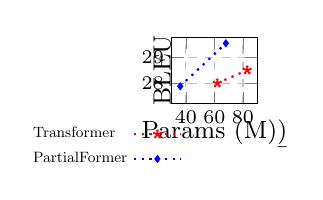
\begin{tikzpicture}[]
  \pgfplotsset{set layers}
     \scriptsize{

    \begin{axis}[
      align=center,
	 at={(0,0)},
      ymajorgrids,
      xmajorgrids,
      grid style=dashed,
      width=0.22\textwidth,
      height=.20\textwidth,
      xlabel={\small \makecell{Params~(M)\b)}},
      ylabel={\small{BLEU}},
      ylabel style={yshift=-2em},xlabel style={yshift=1.0em},
      yticklabel style={/pgf/number format/precision=0,/pgf/number format/fixed zerofill},
      ymin=27.2,ymax=29.8, ytick={ 28, 29},
      xmin=30,xmax=90,xtick={20, 40, 60, 80},
      legend style={
at={(0,0)},
anchor=north east,at={(axis description cs:0,-0.1)}, fill=none, draw=none,yshift=-0.5em,xshift=0.5em,inner sep=0pt,legend plot pos=right,font={\small},cells={anchor=west}, legend columns = 1, ,column sep=0pt}
      ]
    
      
      

       
     
      

    


     
 
      \addplot[dotted, red, mark=star,mark size=.5pt,thick,mark options={solid, fill=red,draw=red,line width=3.25pt}] coordinates { (62, 28.0) (83, 28.51)  
      };\label{Deep_scaling}\addlegendentry{\scalebox{0.6}{Transformer}}

       
      \addplot[dotted, blue,mark=diamond*,mark size=.5pt,thick,mark options={solid, fill=blue,draw=blue,line width=1.25pt}] coordinates {  (36, 27.88)
      (68, 29.56) 


      };\label{PartialFormer}\addlegendentry{\scalebox{0.6}{PartialFormer}}


      
      
      \end{axis}

     
 

      
     }

   
    
  


    
      
      
  \end{tikzpicture}
\vskip -0.1in
    \caption{(a) Scaling Up PartialFormer with Different Methods. (b) Scaling Transformer and PartialFormer with Head Scaling. }
    \label{fig:comparsion_scaling_methods}
\end{figure} 
\begin{table}[t!]
\centering
\renewcommand{\arraystretch}{1}
\centering
\small
\setlength{\tabcolsep}{1pt}

\resizebox{\linewidth}{!}{\begin{tabular}{lrccc}
\toprule

\textbf{Model} &\bf Param 
& \bf Speed (Tok./s) & \bf Memory& \bf BLEU  \\
\midrule
Transformer&  62M &4325 &3.0G& 28.00 \\ 
PartialFormer~(w/o head scaling)& 66M  &3634&3.2G& 28.86 \\
PartialFormer& 68M  &3023&3.3G& \bf 29.56 \\

\bottomrule
\end{tabular}}
    \caption{Efficiency comparison between Transformer and PartialFormer in inference.}
    \label{tab:result_efficiency}
\end{table}


\definecolor{tiffanyblue}{RGB}{129,216,208}
\definecolor{bangdiblue}{RGB}{0,149,182}
\definecolor{kleinblue}{RGB}{0,47,167}
\definecolor{kabuliblue}{RGB}{26,85,153}
\definecolor{purple}{RGB}{138,43,226}
\begin{figure}[t!]
    \centering
  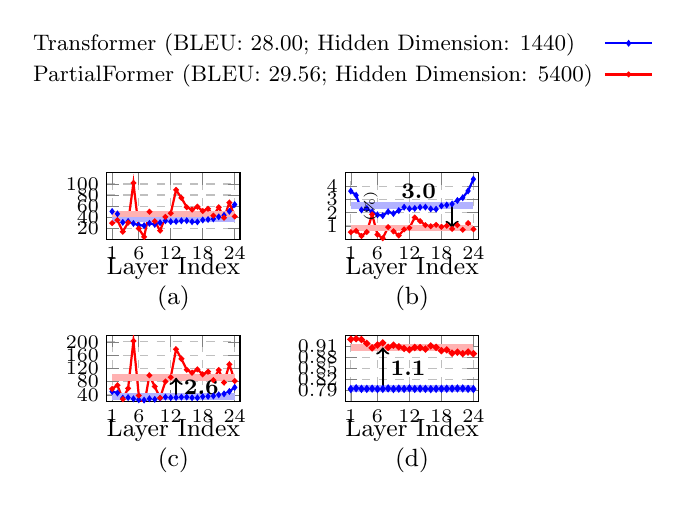
\begin{tikzpicture}[]
  \pgfplotsset{set layers}
     \scriptsize{

    \begin{axis}[
      align=center,
	 at={(0,0)},
      ymajorgrids,
      xmajorgrids,
      grid style=dashed,
      width=0.27\textwidth,
      height=.2\textwidth,
      legend style={at={(0.23,0.08)}, anchor=south west},
      xlabel={\small \makecell{Layer Index \\ (a)}},
      ylabel={\small{}},
      ylabel style={yshift=-2em},xlabel style={yshift=1.0em},
      yticklabel style={/pgf/number format/precision=0,/pgf/number format/fixed zerofill},
      ymin=0,ymax=120, ytick={ 20, 40, 60, 80, 100},
      xmin=0,xmax=25,xtick={1, 6, 12, 18, 24},
      legend style={draw=none,yshift=6.5em,xshift=-5em,inner sep=0pt,legend plot pos=right,font={\small},cells={anchor=west}, legend columns = 1, ,column sep=2pt}
      ]
    
      
      
      \addplot[blue,mark=diamond*,mark size=0.25pt,thick,mark options={fill=blue,draw=blue,line width=1.25pt}] coordinates { (1, 50.397850036621094) (2, 46.05617141723633) (3, 30.716957092285156) (4, 32.27601623535156) (5, 28.592182159423828) (6, 25.675628662109375) (7, 24.729618072509766) (8, 28.869112014770508) (9, 26.933958053588867) (10, 30.077404022216797) (11, 33.576473236083984) (12, 31.970033645629883) (13, 32.3390998840332) (14, 33.447723388671875) (15, 33.69960021972656) (16, 31.835311889648438) (17, 31.542987823486328) (18, 34.97138595581055) (19, 35.815101623535156) (20, 36.96128845214844) (21, 40.59370803833008) (22, 43.48105239868164) (23, 50.58210754394531) (24, 62.86782455444336)


      };\label{baseline}
\addlegendentry{\scalebox{0.9}{Transformer~(BLEU: 28.00; Hidden Dimension: 1440)}}


       
     
      

    


     
 
      \addplot[red, mark=otimes*,mark size=0.25pt,thick,mark options={fill=red,draw=red,line width=1.25pt}] coordinates { (1, 29.44027328491211) (2, 34.75149917602539) (3, 13.85399341583252) (4, 30.174070358276367) (5, 101.7452621459961) (6, 19.441177368164062) (7, 4.418856620788574) (8, 49.83977508544922) (9, 32.83063888549805) (10, 15.632033348083496) (11, 40.52145767211914) (12, 46.91738510131836) (13, 89.28887176513672) (14, 74.86711883544922) (15, 58.14431381225586) (16, 53.80280685424805) (17, 58.88250732421875) (18, 51.280494689941406) (19, 55.328800201416016) (20, 42.71194076538086) (21, 57.96096420288086) (22, 38.90543746948242) (23, 66.41353607177734) (24, 41.248897552490234)
      };
      \addlegendentry{\scalebox{0.9}{PartialFormer~(BLEU: 29.56; Hidden Dimension: 5400)}}

\addplot[blue!30, line width=2pt] coordinates { (1, 35.7504) (24, 35.7504)
      };
      
        \addplot[red!30,line width=2pt] coordinates { (1, 46.1834)  (24, 46.1834)

      };



      
      \end{axis}



     \begin{axis}[
      align=center,
	 at={(0.25\textwidth,0)},
      ymajorgrids,
      xmajorgrids,
      grid style=dashed,
      width=0.27\textwidth,
      height=.2\textwidth,
      legend style={at={(0.23,0.08)}, anchor=south west},
      xlabel={\small \makecell{Layer Index \\ (b)}},
      ylabel={\small{\tiny{(\%)}}},
      ylabel style={yshift=-3em},xlabel style={yshift=1.0em},
      yticklabel style={/pgf/number format/precision=0,/pgf/number format/fixed zerofill},
      ymin=0,ymax=5, ytick={ 1,2, 3,4},
      xmin=0,xmax=25,xtick={1, 6, 12, 18, 24},
      legend style={draw=none,yshift=8em,xshift=0em,inner sep=0pt,legend plot pos=right,font={\small},cells={anchor=west}, legend columns = 1, ,column sep=2pt}
      ]
    
      
      
      \addplot[blue,mark=diamond*,mark size=0.25pt,thick,mark options={fill=blue,draw=blue,line width=1.25pt}] coordinates { 
        (1, 3.628645658493042) (2, 3.3160417079925537) (3, 2.211622714996338) (4, 2.3238747119903564) (5, 2.058638334274292) (6, 1.8486480712890625) (7, 1.7805331945419312) (8, 2.0785739421844482) (9, 1.9392447471618652) (10, 2.1655755043029785) (11, 2.4175031185150146) (12, 2.3018369674682617) (13, 2.328415870666504) (14, 2.4082369804382324) (15, 2.4263756275177) (16, 2.292147159576416) (17, 2.2710978984832764) (18, 2.517946720123291) (19, 2.578690528869629) (20, 2.661208152770996) (21, 2.92274808883667) (22, 3.130636215209961) (23, 3.641909122467041) (24, 4.5264787673950195)

      };\label{baseline}



       
     
      

    


     
 
      \addplot[red, mark=otimes*,mark size=0.25pt,thick,mark options={fill=red,draw=red,line width=1.25pt}] coordinates { (1, 0.5411818623542786) (2, 0.6388141512870789) (3, 0.2546690106391907) (4, 0.5546698570251465) (5, 1.870317816734314) (6, 0.3573746979236603) (7, 0.08122898638248444) (8, 0.916171669960022) (9, 0.6035030484199524) (10, 0.2873530089855194) (11, 0.744879961013794) (12, 0.8624525666236877) (13, 1.641342043876648) (14, 1.3762348890304565) (15, 1.068828821182251) (16, 0.9890232086181641) (17, 1.0823997259140015) (18, 0.9426538944244385) (19, 1.0170739889144897) (20, 0.78514564037323) (21, 1.065460205078125) (22, 0.7151732444763184) (23, 1.2208362817764282) (24, 0.7582511901855469)

      };


\addplot[blue!30, line width=2.5pt] coordinates { (1, 2.5740) (24, 2.5740)
      };
      
        \addplot[red!30,line width=2pt] coordinates { (1, 0.85)  (24, 0.85)

      };

    \draw[<-, thick] (axis cs:20, 0.85) -- (axis cs:20,2.5740) ;
\node[anchor=west,font=\footnotesize] at (axis cs:9, 3.60) {\bf 3.0 };
      
      
      \end{axis}




          \begin{axis}[
      align=center,
	 at={(0,-0.17\textwidth)},
      ymajorgrids,
      xmajorgrids,
      grid style=dashed,
      width=0.27\textwidth,
      height=.2\textwidth,
      legend style={at={(0.23,0.08)}, anchor=south west},
      xlabel={\small \makecell{Layer Index \\ (c)}},
      ylabel={\small{}\tiny{}},
      ylabel style={yshift=-2em},xlabel style={yshift=1.0em},
      yticklabel style={/pgf/number format/precision=0,/pgf/number format/fixed zerofill},
      ymin=20,ymax=220, ytick={ 40, 80, 120, 160, 200},
      xmin=0,xmax=25,xtick={1, 6, 12, 18, 24},
      legend style={draw=none,yshift=8em,xshift=0em,inner sep=0pt,legend plot pos=right,font={\small},cells={anchor=west}, legend columns = 1, ,column sep=2pt}
      ]
    
      
      
      \addplot[blue,mark=diamond*,mark size=0.25pt,thick,mark options={fill=blue,draw=blue,line width=1.25pt}] coordinates { (1, 50.397850036621094) (2, 46.05617141723633) (3, 30.716957092285156) (4, 32.27601623535156) (5, 28.592182159423828) (6, 25.675628662109375) (7, 24.729618072509766) (8, 28.869112014770508) (9, 26.933958053588867) (10, 30.077404022216797) (11, 33.576473236083984) (12, 31.970033645629883) (13, 32.3390998840332) (14, 33.447723388671875) (15, 33.69960021972656) (16, 31.835311889648438) (17, 31.542987823486328) (18, 34.97138595581055) (19, 35.815101623535156) (20, 36.96128845214844) (21, 40.59370803833008) (22, 43.48105239868164) (23, 50.58210754394531) (24, 62.86782455444336)


      };\label{baseline}



       
     
      

    


     
 
      \addplot[red, mark=otimes*,mark size=0.25pt,thick,mark options={fill=red,draw=red,line width=1.25pt}] coordinates { (1, 58.622589111328125) (2, 69.19847869873047) (3, 27.586591720581055) (4, 60.08373260498047) (5, 202.59915161132812) (6, 38.71195983886719) (7, 8.798989295959473) (8, 99.24288940429688) (9, 65.37349700927734) (10, 31.127098083496094) (11, 80.68778228759766) (12, 93.42373657226562) (13, 177.79580688476562) (14, 149.07830810546875) (15, 115.77934265136719) (16, 107.13433837890625) (17, 117.249267578125) (18, 102.11153411865234) (19, 110.17288970947266) (20, 85.04967498779297) (21, 115.41409301757812) (22, 77.47010803222656) (23, 132.24522399902344) (24, 82.13630676269531)

      };


\addplot[blue!30, line width=2.5pt] coordinates { (1, 35.7504) (24, 35.7504)
      };
      
        \addplot[red!30,line width=2.5pt] coordinates { (1, 91.9622)  (24, 91.9622)

      };

    \draw[<-, thick] (axis cs:13, 91.9622) -- (axis cs:13,35.7504) ;
\node[anchor=west,font=\footnotesize] at (axis cs:13, 63.8563) {\bf 2.6 };
      
      
      \end{axis}

    
    \begin{axis}[
	 at={(0.25\textwidth,-0.17\textwidth)},
      ymajorgrids,
      xmajorgrids,
      grid style=dashed,
      width=0.27\textwidth,
      height=.2\textwidth,
      legend style={at={(0.23,0.08)}, anchor=south west},
      xlabel={\small \makecell{Layer Index
      \\ {(d) }}},
      ylabel={\small{}},
      ylabel style={yshift=-1.5em},xlabel style={yshift=1.0em},
      yticklabel style={/pgf/number format/precision=2,/pgf/number format/fixed zerofill},
      ymin=0.76,ymax=0.94, ytick={ 0.79, 0.82, 0.85, 0.88, 0.91},
      xmin=0,xmax=25,xtick={1, 6, 12, 18, 24},
      legend style={yshift=-0.5em,xshift=4em,inner sep=1pt,legend plot pos=right,font={\small},cells={anchor=west}}
      ]


      
      \addplot[blue,mark=diamond*,mark size=0.5pt,thick,mark options={fill=blue,draw=blue,line width=1.25pt}] coordinates { (1,0.7942273020744324)
(2,0.7962304353713989)
(3,0.7946145534515381)
(4,0.7945131659507751)
(5,0.7952606081962585)
(6,0.7940300703048706)
(7,0.7944667339324951)
(8,0.7958396077156067)
(9,0.7942259907722473)
(10,0.7952779531478882)
(11,0.7945087552070618)
(12,0.795943558216095)
(13,0.7943979501724243)
(14,0.7950928211212158)
(15,0.7946134805679321)
(16,0.7939436435699463)
(17,0.7947837114334106)
(18,0.7948220372200012)
(19,0.7949259281158447)
(20,0.7952647805213928)
(21,0.7957655787467957)
(22,0.7956266403198242)
(23,0.7946876287460327)
(24,0.7941218018531799)


      };
     
      

  
      
  \addplot[blue!30,line width=2.5pt] coordinates { (1,0.7949)
(24,0.7949)
      };

     
 
      \addplot[red, mark=otimes*,mark size=0.5pt,thick,mark options={fill=red,draw=red,line width=1.25pt}] coordinates { (1,0.9289955496788025)
(2,0.9303833246231079)
(3,0.9280907511711121)
(4,0.9178294539451599)
(5,0.9058080315589905)
(6,0.9134395718574524)
(7,0.9192654490470886)
(8,0.9071937799453735)
(9,0.9131340980529785)
(10,0.9085556268692017)
(11,0.9041228890419006)
(12,0.9006943106651306)
(13,0.906696081161499)
(14,0.9062924385070801)
(15,0.902535617351532)
(16,0.9111884832382202)
(17,0.9071165323257446)
(18,0.8982360363006592)
(19,0.9003955721855164)
(20,0.8912466764450073)
(21,0.8940209746360779)
(22,0.8901423811912537)
(23,0.894454300403595)
(24,0.8898761868476868)


      };

       \addplot[red!30, line width=2.5pt] coordinates { (1,0.9071)
(24,0.9071)
      };

      \draw[<-, thick] (axis cs:7, 0.9071) -- (axis cs:7,0.7949) ;
\node[anchor=west,font=\footnotesize] at (axis cs:7, 0.8510) {\bf 1.1 };

      \end{axis}

      
     }

   
    
  


    
      
      
  \end{tikzpicture}
\vskip -0.1in
    \caption{Analysis on behaviours of FFNs and head diversity in Transformer and PartialFormer. }
    \label{fig:more_analysis}
    \vspace{-0.25em}
\end{figure} 

\subsection{Analysis on Head Diversity}
\paragraph{Metric.} We select the same metric, namely , as that in \citet{li-etal-2018-multi-head} to measure the diversity among head features. In this metric, a larger value indicates a higher level of diversity.
\paragraph{Results.}
From Figure \ref{fig:more_analysis}(d), we can observe that PartialFormer exhibits more diverse head features compared to the vanilla Transformer. This aligns with previous study~\cite{li-etal-2018-multi-head}, which demonstrates the positive impact of head feature diversity on the Transformer model's performance. Thus, we conclude that the insertion of FFNs into attention mechanism may be a more optimal design.   



\begin{table}[t!]
    \centering
    \renewcommand{\arraystretch}{1}
\centering
\small

\setlength{\tabcolsep}{1pt}
\resizebox{\linewidth}{!}{\begin{tabular}{lrrrrrrccc}
\toprule

\bf Model & -&  &   & & \bf MACs & \bf Param & \bf BLEU  \\
\midrule
Transformer	& 6-6 & 512 & 64	&8-8	&9.9B	&62M	&27.43	 \\
Transformer + LW FFNs	& 6-6 & 512 & 64	&8-8 &	7.7B	&41M	& 26.07
\\
Transformer + PG-FFNs	& 6-6 & 512 & 64	&8-8 &	7.7B	&40M	& 26.82	\\
\bottomrule
\end{tabular}}
    \caption{PG-FFNs offer a compelling alternative to vanilla FFNs. Metrics are reported on WMT'14 En-De. }
    \label{tab:result_PG_FFNs_only}
\end{table}


\section{PG-FFNs: The Perfect Transformer Plug-and-Play Module}
In this section, we emphasized PG-FFNs' plug-and-play adaptability in the Transformer architecture.
\paragraph{Settings.} We replaced the Transformer's FFNs with our PG-FFNs. In the decoder, we exclusively integrated a single PG-FFN for cross-attention, aligning with the original Transformer design. We also created a baseline by using a Transformer with reduced FFN hidden dimensions (384).

\paragraph{Results.}
Table \ref{tab:result_PG_FFNs_only} showcases the superior efficiency of our PG-FFNs. They outperform reduced hidden dimensions in FFNs (26.82 vs. 26.07) with virtually the same computational resources (40M vs. 41M, 7.7B vs. 7.7B), highlighting their potential as a compelling alternative to standard FFNs.








\section{Related Work}
\paragraph{Lightweight Transformers}
Several strands of research have been dedicated to enhancing the parameter efficiency of the Transformer architecture, each taking a distinct approach to the problem at hand. The first category aims to mitigate redundancy directly through architectural innovations, employing more efficient transformation operations~\cite{Mehta2019DeFINEDF,Mehta2021Delight}, integrating disparate yet synergistic patterns~\cite{Wu2020Lite}, or leveraging neural architecture search techniques~\cite{So2019EvolvedTransformer}.
Another avenue of research explores weight sharing as a means of improving parameter efficiency, exemplified by the Universal Transformer's cross-layer parameter sharing strategy~\cite{Dehghani2019UniversalTransformer, reid-etal-2021-subformer-exploring}. Moreover, \citet{li-etal-2022-ode} introduced an ordinary differential equation-inspired weight-sharing approach to achieve higher accuracy in predictions. Different from these work, our study focus on the design of lightweight FFN.




\paragraph{Multi-Branch Transformer}


The multi-branch strategy is widely used in Transformer design. Weighted Transformer~\cite{Ahmed2017WeightedTransformer} employs a multi-branch FFN, while Multi-attentive Transformer~\cite{Fan2020MultibranchAT}, Multi-units Transformer~\cite{yan-etal-2020-multi}, and Multi-Path Transformer~\cite{lin-etal-2022-multi-path} extend this concept to different components of the Transformer. Our PartialFormer can be viewed as a pure multi-branch architecture based on natural subspaces.

\paragraph{Scaling Strategy in Transformer}
Deepening~\cite{bapna-etal-2018-training, wang-etal-2019-learning-deep} and widening~\cite{Vaswani2017transformer, wu2021r} Transformer have been well-acknowledged as two strategies to improve the capacity of Transformer in literature. In this work, PartialFormer adopts two alternative strategies to improve the capacity: specifically, it enhances both the number of attention heads and the dimensions of each head.



\section{Conclusion}

In this paper, we present PartialFormer, a new parameter-efficient Transformer architecture that offers an alternative approach to the design of the lightweight FFN. By employing multiple small FFNs and leveraging matrix factorization techniques, PartialFormer effectively reduces the number of parameters in the FFN. Moreover, we propose two innovative operations to further efficiently enhance the model capabilities. Experimental results across various machine translation tasks showcase the significant performance improvements achieved by PartialFormer, while maintaining comparable parameter consumption. 


 



\section*{Limitations}

Despite the potential advantages of Partialformer in terms of parameter utilization and performance within a limited parameter budget, it is important to note that the existing conclusions regarding its effectiveness have not been thoroughly examined in the context of large-scale datasets and a higher number of parameters. Further research is needed to validate the claims and assess the scalability of Partialformer in more challenging scenarios.



\begin{thebibliography}{49}
\expandafter\ifx\csname natexlab\endcsname\relax\def\natexlab#1{#1}\fi

\bibitem[{Ahmed et~al.(2017)Ahmed, Keskar, and Socher}]{Ahmed2017WeightedTransformer}
Karim Ahmed, Nitish~Shirish Keskar, and Richard Socher. 2017.
\newblock \href {http://arxiv.org/abs/1711.02132} {Weighted transformer network for machine translation}.
\newblock \emph{CoRR}.

\bibitem[{Baevski and Auli(2019)}]{Baevski2019AdaptiveInput}
Alexei Baevski and Michael Auli. 2019.
\newblock \href {https://openreview.net/forum?id=ByxZX20qFQ} {Adaptive input representations for neural language modeling}.
\newblock In \emph{7th International Conference on Learning Representations, {ICLR} 2019, New Orleans, LA, USA, May 6-9, 2019}.

\bibitem[{Bapna et~al.(2018)Bapna, Chen, Firat, Cao, and Wu}]{bapna-etal-2018-training}
Ankur Bapna, Mia Chen, Orhan Firat, Yuan Cao, and Yonghui Wu. 2018.
\newblock \href {https://doi.org/10.18653/v1/D18-1338} {Training deeper neural machine translation models with transparent attention}.
\newblock In \emph{Proceedings of the 2018 Conference on Empirical Methods in Natural Language Processing}, pages 3028--3033, Brussels, Belgium. Association for Computational Linguistics.

\bibitem[{Bonabeau et~al.(1999)Bonabeau, Dorigo, and Theraulaz}]{Bonabeau1999SwarmIntelligence}
Eric Bonabeau, Marco Dorigo, and Guy Theraulaz. 1999.
\newblock \href {https://doi.org/10.1093/oso/9780195131581.001.0001} {\emph{{Swarm Intelligence: From Natural to Artificial Systems}}}.
\newblock Oxford University Press.

\bibitem[{Clark et~al.(2019)Clark, Khandelwal, Levy, and Manning}]{clark-etal-2019-bert}
Kevin Clark, Urvashi Khandelwal, Omer Levy, and Christopher~D. Manning. 2019.
\newblock \href {https://doi.org/10.18653/v1/W19-4828} {What does {BERT} look at? an analysis of {BERT}{'}s attention}.
\newblock In \emph{Proceedings of the 2019 ACL Workshop BlackboxNLP: Analyzing and Interpreting Neural Networks for NLP}, pages 276--286, Florence, Italy. Association for Computational Linguistics.

\bibitem[{Conradt and Roper(2005)}]{conradt2005consensus}
Larissa Conradt and Timothy~J Roper. 2005.
\newblock Consensus decision making in animals.
\newblock \emph{Trends in ecology \& evolution}, 20(8):449--456.

\bibitem[{Couzin(2009)}]{couzin2009collective}
Iain~D Couzin. 2009.
\newblock Collective cognition in animal groups.
\newblock \emph{Trends in cognitive sciences}, 13(1):36--43.

\bibitem[{Dauphin et~al.(2017)Dauphin, Fan, Auli, and Grangier}]{Dauphin2017GLU}
Yann~N. Dauphin, Angela Fan, Michael Auli, and David Grangier. 2017.
\newblock \href {http://proceedings.mlr.press/v70/dauphin17a.html} {Language modeling with gated convolutional networks}.
\newblock In \emph{Proceedings of the 34th International Conference on Machine Learning, {ICML} 2017, Sydney, NSW, Australia, 6-11 August 2017}, volume~70 of \emph{Proceedings of Machine Learning Research}, pages 933--941. {PMLR}.

\bibitem[{Dehghani et~al.(2019)Dehghani, Gouws, Vinyals, Uszkoreit, and Kaiser}]{Dehghani2019UniversalTransformer}
Mostafa Dehghani, Stephan Gouws, Oriol Vinyals, Jakob Uszkoreit, and Lukasz Kaiser. 2019.
\newblock \href {https://openreview.net/forum?id=HyzdRiR9Y7} {Universal transformers}.
\newblock In \emph{7th International Conference on Learning Representations, {ICLR} 2019, New Orleans, LA, USA, May 6-9, 2019}.

\bibitem[{Dong et~al.(2021)Dong, Cordonnier, and Loukas}]{Dong2021PureAttention}
Yihe Dong, Jean{-}Baptiste Cordonnier, and Andreas Loukas. 2021.
\newblock \href {http://proceedings.mlr.press/v139/dong21a.html} {Attention is not all you need: pure attention loses rank doubly exponentially with depth}.
\newblock In \emph{Proceedings of the 38th International Conference on Machine Learning, {ICML} 2021, 18-24 July 2021, Virtual Event}, pages 2793--2803.

\bibitem[{Fan et~al.(2020)Fan, Xie, Xia, Wu, Qin, Li, and Liu}]{Fan2020MultibranchAT}
Yang Fan, Shufang Xie, Yingce Xia, Lijun Wu, Tao Qin, Xiang-Yang Li, and Tie-Yan Liu. 2020.
\newblock Multi-branch attentive transformer.
\newblock \emph{ArXiv}, abs/2006.10270.

\bibitem[{Fan et~al.(2021)Fan, Gong, Liu, Wei, Wang, Jiao, Duan, Zhang, and Huang}]{fan-etal-2021-mask}
Zhihao Fan, Yeyun Gong, Dayiheng Liu, Zhongyu Wei, Siyuan Wang, Jian Jiao, Nan Duan, Ruofei Zhang, and Xuanjing Huang. 2021.
\newblock \href {https://doi.org/10.18653/v1/2021.naacl-main.135} {Mask attention networks: Rethinking and strengthen transformer}.
\newblock In \emph{Proceedings of the 2021 Conference of the North American Chapter of the Association for Computational Linguistics: Human Language Technologies}, pages 1692--1701, Online. Association for Computational Linguistics.

\bibitem[{Ge et~al.(2022)Ge, Chen, and Wei}]{ge-etal-2022-edgeformer}
Tao Ge, Si-Qing Chen, and Furu Wei. 2022.
\newblock \href {https://aclanthology.org/2022.emnlp-main.741} {{E}dge{F}ormer: A parameter-efficient transformer for on-device seq2seq generation}.
\newblock In \emph{Proceedings of the 2022 Conference on Empirical Methods in Natural Language Processing}, pages 10786--10798, Abu Dhabi, United Arab Emirates. Association for Computational Linguistics.

\bibitem[{Gehring et~al.(2017)Gehring, Auli, Grangier, Yarats, and Dauphin}]{Gehring2017convolutionals2s}
Jonas Gehring, Michael Auli, David Grangier, Denis Yarats, and Yann~N. Dauphin. 2017.
\newblock \href {http://proceedings.mlr.press/v70/gehring17a.html} {Convolutional sequence to sequence learning}.
\newblock In \emph{Proceedings of the 34th International Conference on Machine Learning, {ICML} 2017, Sydney, NSW, Australia, 6-11 August 2017}, pages 1243--1252.

\bibitem[{Geva et~al.(2021)Geva, Schuster, Berant, and Levy}]{geva-etal-2021-transformer}
Mor Geva, Roei Schuster, Jonathan Berant, and Omer Levy. 2021.
\newblock \href {https://doi.org/10.18653/v1/2021.emnlp-main.446} {Transformer feed-forward layers are key-value memories}.
\newblock In \emph{Proceedings of the 2021 Conference on Empirical Methods in Natural Language Processing}, pages 5484--5495, Online and Punta Cana, Dominican Republic. Association for Computational Linguistics.

\bibitem[{Gulati et~al.(2020)Gulati, Qin, Chiu, Parmar, Zhang, Yu, Han, Wang, Zhang, Wu, and Pang}]{Gulati-etal-2020-conformer}
Anmol Gulati, James Qin, Chung{-}Cheng Chiu, Niki Parmar, Yu~Zhang, Jiahui Yu, Wei Han, Shibo Wang, Zhengdong Zhang, Yonghui Wu, and Ruoming Pang. 2020.
\newblock \href {https://doi.org/10.21437/Interspeech.2020-3015} {Conformer: Convolution-augmented transformer for speech recognition}.
\newblock In \emph{Interspeech 2020, 21st Annual Conference of the International Speech Communication Association, Virtual Event, Shanghai, China, 25-29 October 2020}, pages 5036--5040. {ISCA}.

\bibitem[{He et~al.(2021)He, Ravula, Kanagal, and Ainslie}]{he-etal-2021-realformer}
Ruining He, Anirudh Ravula, Bhargav Kanagal, and Joshua Ainslie. 2021.
\newblock \href {https://doi.org/10.18653/v1/2021.findings-acl.81} {{R}eal{F}ormer: Transformer likes residual attention}.
\newblock In \emph{Findings of the Association for Computational Linguistics: ACL-IJCNLP 2021}, pages 929--943, Online. Association for Computational Linguistics.

\bibitem[{Lan et~al.(2020)Lan, Chen, Goodman, Gimpel, Sharma, and Soricut}]{Lan2020ALBERT}
Zhenzhong Lan, Mingda Chen, Sebastian Goodman, Kevin Gimpel, Piyush Sharma, and Radu Soricut. 2020.
\newblock \href {https://openreview.net/forum?id=H1eA7AEtvS} {{ALBERT:} {A} lite {BERT} for self-supervised learning of language representations}.
\newblock In \emph{8th International Conference on Learning Representations, {ICLR} 2020, Addis Ababa, Ethiopia, April 26-30, 2020}.

\bibitem[{Li et~al.(2022)Li, Du, Zhou, Jing, Zhou, Zeng, Xiao, Zhu, Liu, and Zhang}]{li-etal-2022-ode}
Bei Li, Quan Du, Tao Zhou, Yi~Jing, Shuhan Zhou, Xin Zeng, Tong Xiao, JingBo Zhu, Xuebo Liu, and Min Zhang. 2022.
\newblock \href {https://doi.org/10.18653/v1/2022.acl-long.571} {{ODE} transformer: An ordinary differential equation-inspired model for sequence generation}.
\newblock In \emph{Proceedings of the 60th Annual Meeting of the Association for Computational Linguistics (Volume 1: Long Papers)}, pages 8335--8351, Dublin, Ireland. Association for Computational Linguistics.

\bibitem[{Li et~al.(2018)Li, Tu, Yang, Lyu, and Zhang}]{li-etal-2018-multi-head}
Jian Li, Zhaopeng Tu, Baosong Yang, Michael~R. Lyu, and Tong Zhang. 2018.
\newblock \href {https://doi.org/10.18653/v1/D18-1317} {Multi-head attention with disagreement regularization}.
\newblock In \emph{Proceedings of the 2018 Conference on Empirical Methods in Natural Language Processing}, pages 2897--2903, Brussels, Belgium. Association for Computational Linguistics.

\bibitem[{Lin(2004)}]{lin-2004-rouge}
Chin-Yew Lin. 2004.
\newblock \href {https://aclanthology.org/W04-1013} {{ROUGE}: A package for automatic evaluation of summaries}.
\newblock In \emph{Text Summarization Branches Out}, pages 74--81, Barcelona, Spain. Association for Computational Linguistics.

\bibitem[{Lin et~al.(2022)Lin, Zhou, Li, Ma, Xiao, and Zhu}]{lin-etal-2022-multi-path}
Ye~Lin, Shuhan Zhou, Yanyang Li, Anxiang Ma, Tong Xiao, and Jingbo Zhu. 2022.
\newblock \href {https://aclanthology.org/2022.findings-emnlp.414} {Multi-path transformer is better: A case study on neural machine translation}.
\newblock In \emph{Findings of the Association for Computational Linguistics: EMNLP 2022}, pages 5646--5656, Abu Dhabi, United Arab Emirates. Association for Computational Linguistics.

\bibitem[{Lu et~al.(2019)Lu, Li, He, Sun, Dong, Qin, Wang, and Liu}]{Lu-etal-2020-Macaron}
Yiping Lu, Zhuohan Li, Di~He, Zhiqing Sun, Bin Dong, Tao Qin, Liwei Wang, and Tie{-}Yan Liu. 2019.
\newblock \href {http://arxiv.org/abs/1906.02762} {Understanding and improving transformer from a multi-particle dynamic system point of view}.
\newblock \emph{CoRR}, abs/1906.02762.

\bibitem[{Ma et~al.(2018)Ma, Zhang, Zheng, and Sun}]{Ningning2018shufflenetv2}
Ningning Ma, Xiangyu Zhang, Hai-Tao Zheng, and Jian Sun. 2018.
\newblock \href {https://doi.org/10.1007/978-3-030-01264-9_8} {Shufflenet v2: Practical guidelines for efficient cnn architecture design}.
\newblock In \emph{Computer Vision – ECCV 2018: 15th European Conference, Munich, Germany, September 8–14, 2018, Proceedings, Part XIV}, page 122–138, Berlin, Heidelberg. Springer-Verlag.

\bibitem[{Ma et~al.(2022)Ma, Zhou, Kong, He, Gui, Neubig, May, and Zettlemoyer}]{Ma2022mega}
Xuezhe Ma, Chunting Zhou, Xiang Kong, Junxian He, Liangke Gui, Graham Neubig, Jonathan May, and Luke Zettlemoyer. 2022.
\newblock \href {https://doi.org/10.48550/arXiv.2209.10655} {Mega: Moving average equipped gated attention}.
\newblock \emph{CoRR}.

\bibitem[{Mehta et~al.(2021)Mehta, Ghazvininejad, Iyer, Zettlemoyer, and Hajishirzi}]{Mehta2021Delight}
Sachin Mehta, Marjan Ghazvininejad, Srinivasan Iyer, Luke Zettlemoyer, and Hannaneh Hajishirzi. 2021.
\newblock \href {https://openreview.net/forum?id=ujmgfuxSLrO} {Delight: Deep and light-weight transformer}.
\newblock In \emph{9th International Conference on Learning Representations, {ICLR} 2021, Virtual Event, Austria, May 3-7, 2021}.

\bibitem[{Mehta et~al.(2019)Mehta, Koncel-Kedziorski, Rastegari, and Hajishirzi}]{Mehta2019DeFINEDF}
Sachin Mehta, Rik Koncel-Kedziorski, Mohammad Rastegari, and Hannaneh Hajishirzi. 2019.
\newblock Define: Deep factorized input word embeddings for neural sequence modeling.
\newblock \emph{ArXiv}, abs/1911.12385.

\bibitem[{Michel et~al.(2019)Michel, Levy, and Neubig}]{michel2019sixteen}
Paul Michel, Omer Levy, and Graham Neubig. 2019.
\newblock Are sixteen heads really better than one?
\newblock \emph{Advances in neural information processing systems}, 32.

\bibitem[{Nguyen et~al.(2022)Nguyen, Nguyen, Do, Nguyen, Saragadam, Pham, Khuong, Ho, and Osher}]{nguyen2022improving}
Tan~Minh Nguyen, Tam~Minh Nguyen, Hai~Ngoc Do, Khai Nguyen, Vishwanath Saragadam, Minh Pham, Nguyen~Duy Khuong, Nhat Ho, and Stanley Osher. 2022.
\newblock \href {https://openreview.net/forum?id=0VFQhPGF1M3} {Improving transformer with an admixture of attention heads}.
\newblock In \emph{Advances in Neural Information Processing Systems}.

\bibitem[{Ott et~al.(2019)Ott, Edunov, Baevski, Fan, Gross, Ng, Grangier, and Auli}]{ott-etal-2019-fairseq}
Myle Ott, Sergey Edunov, Alexei Baevski, Angela Fan, Sam Gross, Nathan Ng, David Grangier, and Michael Auli. 2019.
\newblock \href {https://doi.org/10.18653/v1/N19-4009} {fairseq: A fast, extensible toolkit for sequence modeling}.
\newblock In \emph{Proceedings of the 2019 Conference of the North {A}merican Chapter of the Association for Computational Linguistics (Demonstrations)}, pages 48--53, Minneapolis, Minnesota. Association for Computational Linguistics.

\bibitem[{Papineni et~al.(2002)Papineni, Roukos, Ward, and Zhu}]{papineni-etal-2002-bleu}
Kishore Papineni, Salim Roukos, Todd Ward, and Wei-Jing Zhu. 2002.
\newblock \href {https://doi.org/10.3115/1073083.1073135} {{B}leu: a method for automatic evaluation of machine translation}.
\newblock In \emph{Proceedings of the 40th Annual Meeting of the Association for Computational Linguistics}, pages 311--318, Philadelphia, Pennsylvania, USA. Association for Computational Linguistics.

\bibitem[{Post(2018)}]{post-2018-call}
Matt Post. 2018.
\newblock \href {https://doi.org/10.18653/v1/W18-6319} {A call for clarity in reporting {BLEU} scores}.
\newblock In \emph{Proceedings of the Third Conference on Machine Translation: Research Papers}, pages 186--191, Brussels, Belgium. Association for Computational Linguistics.

\bibitem[{Rei et~al.(2022)Rei, C.~de Souza, Alves, Zerva, Farinha, Glushkova, Lavie, Coheur, and Martins}]{rei-etal-2022-comet}
Ricardo Rei, Jos{\'e}~G. C.~de Souza, Duarte Alves, Chrysoula Zerva, Ana~C Farinha, Taisiya Glushkova, Alon Lavie, Luisa Coheur, and Andr{\'e} F.~T. Martins. 2022.
\newblock \href {https://aclanthology.org/2022.wmt-1.52} {{COMET}-22: Unbabel-{IST} 2022 submission for the metrics shared task}.
\newblock In \emph{Proceedings of the Seventh Conference on Machine Translation (WMT)}, pages 578--585, Abu Dhabi, United Arab Emirates (Hybrid). Association for Computational Linguistics.

\bibitem[{Reid et~al.(2021)Reid, Marrese-Taylor, and Matsuo}]{reid-etal-2021-subformer-exploring}
Machel Reid, Edison Marrese-Taylor, and Yutaka Matsuo. 2021.
\newblock \href {https://doi.org/10.18653/v1/2021.findings-emnlp.344} {Subformer: Exploring weight sharing for parameter efficiency in generative transformers}.
\newblock In \emph{Findings of the Association for Computational Linguistics: EMNLP 2021}, pages 4081--4090, Punta Cana, Dominican Republic. Association for Computational Linguistics.

\bibitem[{Sennrich et~al.(2016)Sennrich, Haddow, and Birch}]{sennrich-etal-2016-neural}
Rico Sennrich, Barry Haddow, and Alexandra Birch. 2016.
\newblock \href {https://doi.org/10.18653/v1/P16-1162} {Neural machine translation of rare words with subword units}.
\newblock In \emph{Proceedings of the 54th Annual Meeting of the Association for Computational Linguistics (Volume 1: Long Papers)}, pages 1715--1725, Berlin, Germany. Association for Computational Linguistics.

\bibitem[{Shaw et~al.(2018)Shaw, Uszkoreit, and Vaswani}]{shaw-etal-2018-self}
Peter Shaw, Jakob Uszkoreit, and Ashish Vaswani. 2018.
\newblock \href {https://doi.org/10.18653/v1/N18-2074} {Self-attention with relative position representations}.
\newblock In \emph{Proceedings of the 2018 Conference of the North {A}merican Chapter of the Association for Computational Linguistics: Human Language Technologies, Volume 2 (Short Papers)}, pages 464--468, New Orleans, Louisiana. Association for Computational Linguistics.

\bibitem[{Shazeer(2020)}]{shazeer2020glu}
Noam Shazeer. 2020.
\newblock Glu variants improve transformer.
\newblock \emph{arXiv preprint arXiv:2002.05202}.

\bibitem[{So et~al.(2019)So, Le, and Liang}]{So2019EvolvedTransformer}
David~R. So, Quoc~V. Le, and Chen Liang. 2019.
\newblock \href {http://proceedings.mlr.press/v97/so19a.html} {The evolved transformer}.
\newblock In \emph{Proceedings of the 36th International Conference on Machine Learning, {ICML} 2019, 9-15 June 2019, Long Beach, California, {USA}}, pages 5877--5886.

\bibitem[{Sutskever et~al.(2014)Sutskever, Vinyals, and Le}]{Sutskever2014sequence2sequence}
Ilya Sutskever, Oriol Vinyals, and Quoc~V. Le. 2014.
\newblock \href {https://proceedings.neurips.cc/paper/2014/hash/a14ac55a4f27472c5d894ec1c3c743d2-Abstract.html} {Sequence to sequence learning with neural networks}.
\newblock In \emph{Advances in Neural Information Processing Systems 27: Annual Conference on Neural Information Processing Systems 2014, December 8-13 2014, Montreal, Quebec, Canada}, pages 3104--3112.

\bibitem[{Tan and Le(2019)}]{tan2019efficientnet}
Mingxing Tan and Quoc Le. 2019.
\newblock Efficientnet: Rethinking model scaling for convolutional neural networks.
\newblock In \emph{International conference on machine learning}, pages 6105--6114. PMLR.

\bibitem[{Tran et~al.(2021)Tran, Bhosale, Cross, Koehn, Edunov, and Fan}]{tran-etal-2021-facebook}
Chau Tran, Shruti Bhosale, James Cross, Philipp Koehn, Sergey Edunov, and Angela Fan. 2021.
\newblock \href {https://aclanthology.org/2021.wmt-1.19} {{F}acebook {AI}{'}s {WMT}21 news translation task submission}.
\newblock In \emph{Proceedings of the Sixth Conference on Machine Translation}, pages 205--215, Online. Association for Computational Linguistics.

\bibitem[{Vaswani et~al.(2017)Vaswani, Shazeer, Parmar, Uszkoreit, Jones, Gomez, Kaiser, and Polosukhin}]{Vaswani2017transformer}
Ashish Vaswani, Noam Shazeer, Niki Parmar, Jakob Uszkoreit, Llion Jones, Aidan~N. Gomez, Lukasz Kaiser, and Illia Polosukhin. 2017.
\newblock \href {https://proceedings.neurips.cc/paper/2017/hash/3f5ee243547dee91fbd053c1c4a845aa-Abstract.html} {Attention is all you need}.
\newblock In \emph{Advances in Neural Information Processing Systems 30: Annual Conference on Neural Information Processing Systems 2017, December 4-9, 2017, Long Beach, CA, {USA}}, pages 5998--6008.

\bibitem[{Voita et~al.(2019)Voita, Talbot, Moiseev, Sennrich, and Titov}]{voita-etal-2019-analyzing}
Elena Voita, David Talbot, Fedor Moiseev, Rico Sennrich, and Ivan Titov. 2019.
\newblock \href {https://doi.org/10.18653/v1/P19-1580} {Analyzing multi-head self-attention: Specialized heads do the heavy lifting, the rest can be pruned}.
\newblock In \emph{Proceedings of the 57th Annual Meeting of the Association for Computational Linguistics}, pages 5797--5808, Florence, Italy. Association for Computational Linguistics.

\bibitem[{Wang et~al.(2022)Wang, Zheng, Chen, and Wang}]{Wang2022AntiOversmoothing}
Peihao Wang, Wenqing Zheng, Tianlong Chen, and Zhangyang Wang. 2022.
\newblock \href {https://openreview.net/forum?id=O476oWmiNNp} {Anti-oversmoothing in deep vision transformers via the fourier domain analysis: From theory to practice}.
\newblock In \emph{The Tenth International Conference on Learning Representations, {ICLR} 2022, Virtual Event, April 25-29, 2022}.

\bibitem[{Wang et~al.(2019)Wang, Li, Xiao, Zhu, Li, Wong, and Chao}]{wang-etal-2019-learning-deep}
Qiang Wang, Bei Li, Tong Xiao, Jingbo Zhu, Changliang Li, Derek~F. Wong, and Lidia~S. Chao. 2019.
\newblock \href {https://doi.org/10.18653/v1/P19-1176} {Learning deep transformer models for machine translation}.
\newblock In \emph{Proceedings of the 57th Annual Meeting of the Association for Computational Linguistics}, pages 1810--1822, Florence, Italy. Association for Computational Linguistics.

\bibitem[{Wu et~al.(2021)Wu, Li, Wang, Meng, Qin, Chen, Zhang, Liu et~al.}]{wu2021r}
Lijun Wu, Juntao Li, Yue Wang, Qi~Meng, Tao Qin, Wei Chen, Min Zhang, Tie-Yan Liu, et~al. 2021.
\newblock R-drop: Regularized dropout for neural networks.
\newblock \emph{Advances in Neural Information Processing Systems}, 34:10890--10905.

\bibitem[{Wu et~al.(2020)Wu, Liu, Lin, Lin, and Han}]{Wu2020Lite}
Zhanghao Wu, Zhijian Liu, Ji~Lin, Yujun Lin, and Song Han. 2020.
\newblock \href {https://openreview.net/forum?id=ByeMPlHKPH} {Lite transformer with long-short range attention}.
\newblock In \emph{8th International Conference on Learning Representations, {ICLR} 2020, Addis Ababa, Ethiopia, April 26-30, 2020}.

\bibitem[{Yan et~al.(2020)Yan, Meng, and Zhou}]{yan-etal-2020-multi}
Jianhao Yan, Fandong Meng, and Jie Zhou. 2020.
\newblock \href {https://doi.org/10.18653/v1/2020.emnlp-main.77} {Multi-unit transformers for neural machine translation}.
\newblock In \emph{Proceedings of the 2020 Conference on Empirical Methods in Natural Language Processing (EMNLP)}, pages 1047--1059, Online. Association for Computational Linguistics.

\bibitem[{Zhang et~al.(2022)Zhang, Lin, Liu, Li, Sun, and Zhou}]{zhang-etal-2022-moefication}
Zhengyan Zhang, Yankai Lin, Zhiyuan Liu, Peng Li, Maosong Sun, and Jie Zhou. 2022.
\newblock \href {https://doi.org/10.18653/v1/2022.findings-acl.71} {{M}o{E}fication: Transformer feed-forward layers are mixtures of experts}.
\newblock In \emph{Findings of the Association for Computational Linguistics: ACL 2022}, pages 877--890, Dublin, Ireland. Association for Computational Linguistics.

\end{thebibliography}
 \bibliographystyle{acl_natbib}

\newpage

\appendix
\section{Detailed Setups of Experiments}
\label{sec:detailed_settup}

\subsection{Dataset}
Table \ref{tab:dataset_deatails} displays the statistics of all the 9 translation task.

\subsection{Training Details}
Table \ref{tab:training_ende_enfr_enro} and \ref{tab:training_wmt17} exhibits the training details on all translation tasks.









\section{Implementation of Previous State-of-the-art Methods}
The accuracy of fairseq-based translation results can vary due to tokenization methods and other factors. To address fairness concerns, we re-implemented three state-of-the-art approaches in our codebase. To ensure absolute fairness, we employed the identical training strategy and data usage as in our PartialFormer model.

\paragraph{Data.} The dataset is sourced from Google's open release, featuring BPE operations totaling 32K. 
\paragraph{Training Strategy.} Our training strategy is the same as that of \citet{wang-etal-2019-learning-deep}, where 0.002 learning rate, 16000 warmup steps, pre-norm, relu\_dropout=0.1, attention dropout=0.1, 4096 tokens per GPUs (8 GPUs) and update the parameters every 2 steps.


\paragraph{Results.}
We can see that recent methods like Mega-Softmax and DMAN do not perform well with our training approach due to their longer training requirements. Thus, we believe that citing the results from their original paper might be a better way.



\section{Ablation on Design of Decoder}
\label{sec_compare_decoder}

The design of the Decoder is a crucial component of the Transformer architecture due to its direct association with decoding. We evaluated three configurations: 1) Integrating PG-FFNs into both the decoder's self-attention and cross-attention, while halving the hidden dimension, 2) Incorporating PG-FFNs solely into the decoder's cross-attention, and 3) Incorporating PG-FFNs solely into the decoder's self-attention. 

Table \ref{tab:result_PG_FFNs_compare} exhibited the results on the WMT'14 En-De task. Our observations are as follows: 1) The first configuration yields the best performance, aligning with the insights from \citet{Gulati-etal-2020-conformer, Lu-etal-2020-Macaron}, 2) Using a single PG-FFN in each layer also delivers commendable results with a score of 29.21, and 3) Excluding PG-FFNs from the decoder's cross-attention results in erratic training, which is expected since there are no FFNs to handle the cross-attention features.



\section{Metric Definition}

\subsection{Measurement of Head Diversity}
Following \citet{li-etal-2018-multi-head}, we measure the head diversity as follows:

    
During evaluation, we calculate the metric on all samples and average the values to obtain the final result.






\begin{table}[ht!]
\centering
\setlength{\tabcolsep}{1.5pt}
\begin{tabular}{lrrrcc}
\toprule
\multirow{2}{*}{\textbf{Dataset}}& \multicolumn{3}{c}{\textbf{Sentence}}& \multirow{2}{*}{\textbf{BPE}} & \multirow{2}{*}{\textbf{Vocab}}  \\
\cmidrule{2-4}
& \textbf{Train} & \textbf{Dev} & \textbf{Test} &  &  \\
\midrule
WMT'14 En-De & 4.5M&2999&3003 & 32K & 34040\\
WMT'14 En-Fr & 36M&26815&3003 & 32K & 37288\\
WMT'16 En-Ro  & 0.6M&1999& 1999 &  20K&  19064\\
WMT'17 En-De & 5.9M&7998&3004 & 32K & 35488\\
WMT'17 De-En & 5.9M&7998&3004 & 32K & 35448\\
WMT'17 En-Fi  & 2.7M&4225& 3002 &  32K&  32584\\
WMT'17 Fi-En  & 2.7M&4225& 3002 &  32K&  32584\\
WMT'17 En-Lv  & 4.5M&2003& 2001 &  32K&  32368\\
WMT'17 Lv-En  & 4.5M&2003& 2001 &  32K&  32368\\
\bottomrule
\end{tabular}
\caption{The details of datasets of 9 translation tasks.}
\label{tab:dataset_deatails}
\end{table}








\begin{table}[ht!]
\centering
\small
\setlength{\tabcolsep}{1.5pt}
\begin{tabular}{lccccc}
\toprule
& \bf En-De & \bf En-Ro & \bf En-Fr   \\
\midrule
GPUs & 8 & 4 & 8 \\
Batch Size & 4096 &4096 & 4096 \\
Update Frequency & 2 & 1 & 8 &\\
Optimer & Adam  & Adam  & Adam  \\
{}  & (0.9, 0.997)  & (0.9, 0.997)  & (0.9, 0.997)   \\
LR & 0.0020 &0.0020 & 0.0020 \\
LR scheduler  & inverse sqrt &inverse sqrt & inverse sqrt \\
Initial LR & 1 &1 & 1  \\
Total updates & 50K & 25K& 100K \\
Warmup updates & 16000 &8000 & 16000  \\
Weight decay & 0.0000 &0.0000 &  0.0000\\
Label smoothing & 0.1 & 0.1 & 0.1 \\
Dropout & 0.1  & 0.1  & 0.1  \\
Attention dropout & 0.1 & 0.1 & 0.1 \\
ReLU dropout & 0.1 & 0.1 & 0.1 \\
\toprule
\end{tabular}
\caption{The training setups of WMT'14 En-De, WMT'16 En-Ro and WMT'14 En-Fr tasks.  }
\label{tab:training_ende_enfr_enro}
\end{table}



\begin{table}[ht!]
\centering
\small
\setlength{\tabcolsep}{1pt}
\resizebox{\linewidth}{!}{\begin{tabular}{lccccc}
\toprule
& \bf En-\{De, Lv\} & \bf \{De, Lv\}-En & \bf En-Fi  & \bf  Fi-En    \\
\midrule
GPUs & 8 & 8 & 8 & 8 \\
Batch Size & 4096 &4096 & 4096 & 4096 \\
Update Frequency & 2 & 1 & 1 & 4 \\
Optimer & Adam  & Adam  & Adam & Adam  \\
{}  & (0.9, 0.997)  & (0.9, 0.997)  & (0.9, 0.997) & (0.9, 0.997)   \\
LR & 0.0020 &0.0020 & 0.0020 & 0.0020 \\
LR scheduler  & inverse sqrt &inverse sqrt & inverse sqrt & inverse sqrt \\
Initial LR & 1 &1 & 1 & 1  \\
Total updates & 50K/17K & 50K/17K& 40K & 10K\\
Warmup updates & 16000 &16000 & 16000 & 16000  \\
Weight decay & 0.0000 &0.0000 &  0.0000 &  0.0000\\
Label smoothing & 0.1 & 0.1 & 0.1 & 0.1 \\
Dropout & 0.1  & 0.1  & 0.1  & 0.1  \\
Attention dropout & 0.1 & 0.1 & 0.1 & 0.1 \\
ReLU dropout & 0.1 & 0.1 & 0.1 & 0.1 \\
\toprule
\end{tabular}}
\caption{The training setups of WMT'17 benchmark.  }
\label{tab:training_wmt17}
\end{table}



\begin{table}[ht]
\renewcommand{\arraystretch}{1}
\centering
\small
\setlength{\tabcolsep}{1.5pt}

\begin{tabular}{lrc}
\toprule

\textbf{Model} 
& \bf Param  & \bf BLEU\\
\midrule
Mega-Softmax (Post-Norm) &	64M	& 27.87 \\
Mega-Softmax (Pre-Norm) &	64M	& 28.11\\
ODE Transformer &62M &	29.03 \\
\bottomrule
\end{tabular}

    \caption{Results of state-of-the-art models employing the same training strategy and data for the En-De task.}
    \label{tab:result_comparision_small}
\end{table}



\begin{table}[t!]
    \centering
    \renewcommand{\arraystretch}{1}
\centering
\small

\setlength{\tabcolsep}{1pt}
\begin{tabular}{lrrr}
\toprule
\bf Model  & \bf Param & \bf BLEU  \\
\midrule
PartialFormer		&68M	&29.56	 \\
\quad -PGFFNs in decoder self-AFFN		 &66M	& 29.21
\\
\quad -PGFFNs in decoder cross-AFFN		 &66M	& Failed \\
\bottomrule
\end{tabular}
    \caption{\textbf{Utilizing PG-FFNs in both the decoder's self-attention and cross-attention mechanisms is a preferable option.} BLEU points are reported in WMT'14 En-De task. }
    \label{tab:result_PG_FFNs_compare}
\end{table}











\begin{table}[t!]
\renewcommand{\arraystretch}{1}
\centering
\small
\setlength{\tabcolsep}{1.5pt}

\resizebox{0.9\linewidth}{!}{\begin{tabular}{lrc}
\toprule

\textbf{Model} 
& \bf Param  & \bf BLEU\\
\midrule
\textsc{Delight}~\cite{Mehta2021Delight} & 23M &  26.70\\
EdgeFormer~\cite{ge-etal-2022-edgeformer} & - &  26.90\\
Lite Transformer~\cite{Wu2020Lite} & - &  26.50\\
PartialFormer & 27M & \bf 27.50\\
\midrule
Evolved Transformer~\cite{So2019EvolvedTransformer} & 48M & 27.70 \\
\textsc{Delight}~\cite{Mehta2021Delight} & 37M &  27.60\\
ODE Transformer~\cite{li-etal-2022-ode} & 37M &  28.24\\
PartialFormer & 36M & \bf 28.35\\

\bottomrule
\end{tabular}}

    \caption{Comparison with state-of-the-art models of smaller capacities on the En-De task. }
    \label{tab:result_comparision_small}
\end{table}


\begin{table}[ht!]
    \centering
    \renewcommand{\arraystretch}{1}
\centering
\small
\setlength{\tabcolsep}{3pt}

\begin{tabular}{cccrcr}
\toprule
 \bf  & \bf  & \bf Param & \bf BLEU \\

\midrule
RPR  &MHSA &62M & 35.76  \\
\bottomrule
\end{tabular}
\caption{Results of several PartialFormer variants on the En-De task.}
\label{tab:PartialFormer_A_G_VARIANTS}
\end{table}







\section{More Comparison with Previous Lightweight Transformer}


Table \ref{tab:result_comparision_small} presents a comprehensive comparison of previous lightweight Transformer models on the En-De task's test set, with a specific focus on operating within a smaller parameter budget. The results prominently showcase the outstanding performance of PartialFormer, even when faced with constraints on model capacity. This outcome further emphasizes the superior capabilities of PartialFormer in scenarios with limited resources.

\section{PartialFormer with Different  for Small Dataset}
\label{sec:partial_different_A_G}
Table \ref{tab:PartialFormer_A_G_VARIANTS} showcases the results of PartialFormer on the WMT'16 En-Ro task, a small-scale translation dataset, specifically when  is calculated using local attention~\cite{shaw-etal-2018-self}. Notably, these results reveal that by adopting such an approach, PartialFormer achieves an impressive BLEU score of 35.76. We hope this can shed lights on the area of model integration.
\section{PartialFormer with GLU and Weight Sharing}

 

In this section, we investigate the integration of PartialFormer with two prominent techniques to enhance parameter efficiency: 1) the weight sharing method~\cite{Lan2020ALBERT}, and 2) gated linear units~\cite{Dauphin2017GLU}. To ensure the utilization of the latest advancements, we employ a state-of-the-art weight sharing method called ODE Transformer~\cite{li-etal-2022-ode}, known for its effectiveness in promoting parameter efficiency in Transformer architectures. Additionally, we incorporate Swi-GLU~\cite{shazeer2020glu}, a widely adopted GLU-variant that has served as a foundational component in numerous expressive Transformer architectures.


Table \ref{tab:PartialFormer_GLU_VARIANTS} displays the results of combining PartialFormer with weight sharing and gated linear units. Despite the integration of these two techniques, the performance gains are marginal. This could be attributed to the fact that PartialFormer already possesses high parameter efficiency, leaving little room for additional enhancements from other technologies. In other words, PartialFormer is inherently a high parameter efficiency architecture.



\section{Analysis on Token Uniformity}
\label{sec:analysis_tu}
Following \cite{Dong2021PureAttention, Wang2022AntiOversmoothing}, we measure the token uniformity among token representations. We use pearson correlation to compute it.


From Figure \ref{fig:analysis_tu}, we can observe that PartialFormer owns a lower token uniformity among token representations than the vanilla Transformer, revealing that PartialFormer can benefit from depth scaling efficiently~\cite{Dong2021PureAttention, Wang2022AntiOversmoothing}.



\begin{table}[t!]
    \centering
    \renewcommand{\arraystretch}{1}
\centering
\small
\setlength{\tabcolsep}{2pt}

\resizebox{0.9\linewidth}{!}{\begin{tabular}{lcrc}
\toprule
\bf Model & \bf Param & \bf BLEU \\

\midrule
PartialFormer &67M & 29.56 \\
PartialFormer + Weight Sharing &67M & 29.71 \\
GLU-based PartialFormer  &67M & 29.67 \\
\bottomrule
\end{tabular}}
\caption{Results of PartialFormer variants on the En-De task.}
\label{tab:PartialFormer_GLU_VARIANTS}
\end{table}



\definecolor{tiffanyblue}{RGB}{129,216,208}
\definecolor{bangdiblue}{RGB}{0,149,182}
\definecolor{kleinblue}{RGB}{0,47,167}
\definecolor{kabuliblue}{RGB}{26,85,153}
\definecolor{purple}{RGB}{138,43,226}
\begin{figure}[ht!]
    \centering
  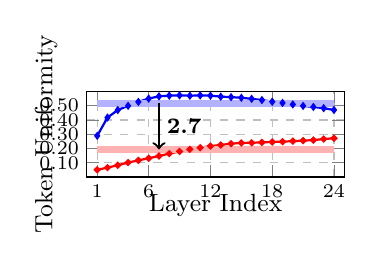
\begin{tikzpicture}[]
  \pgfplotsset{set layers}
     \scriptsize{

    \begin{axis}[
	 at={(0.66\textwidth,0)},
      ymajorgrids,
      xmajorgrids,
      grid style=dashed,
      width=0.40\textwidth,
      height=.22\textwidth,
      legend style={at={(0.23,0.08)}, anchor=south west},
      xlabel={\small \makecell{Layer Index
      \\ }},
      ylabel={\small{Token Uniformity}},
      ylabel style={yshift=-1.5em},xlabel style={yshift=1.0em},
      yticklabel style={/pgf/number format/precision=2,/pgf/number format/fixed zerofill},
      ymin=0,ymax=0.6, ytick={ 0.1, 0.2, 0.3, 0.4, 0.5},
      xmin=0,xmax=25,xtick={1, 6, 12, 18, 24},
      legend style={yshift=-0.5em,xshift=4em,inner sep=1pt,legend plot pos=right,font={\footnotesize},cells={anchor=west}}
      ]


      
      \addplot[blue,mark=diamond*,mark size=0.5pt,thick,mark options={fill=blue,draw=blue,line width=1.25pt}] coordinates { (1, 0.28883352875709534) (2, 0.41732001304626465) (3, 0.4699432849884033) (4, 0.4995066225528717) (5, 0.5271627306938171) (6, 0.5504211783409119) (7, 0.5659817457199097) (8, 0.5709900259971619) (9, 0.5731505751609802) (10, 0.570284366607666) (11, 0.5726948976516724) (12, 0.5708319544792175) (13, 0.563860297203064) (14, 0.5604643225669861) (15, 0.5560687780380249) (16, 0.5486728549003601) (17, 0.5399861335754395) (18, 0.5283432602882385) (19, 0.5198920965194702) (20, 0.5089938640594482) (21, 0.498872846364975) (22, 0.49158498644828796) (23, 0.48306941986083984) (24, 0.47021931409835815)

      };



      \addplot[blue!30,line width=2.5pt] coordinates { (1, 0.5186) (24, 0.5186)

      };

    


     
 
      \addplot[red, mark=otimes*,mark size=0.5pt,thick,mark options={fill=red,draw=red,line width=1.25pt}] coordinates { (1, 0.05046646296977997) (2, 0.06599926948547363) (3, 0.08231858164072037) (4, 0.10168235003948212) (5, 0.11680775880813599) (6, 0.1316044181585312) (7, 0.14767728745937347) (8, 0.16397510468959808) (9, 0.17946700751781464) (10, 0.19437670707702637) (11, 0.2057010680437088) (12, 0.21689032018184662) (13, 0.2251075953245163) (14, 0.23383928835391998) (15, 0.2391471564769745) (16, 0.24002841114997864) (17, 0.24297945201396942) (18, 0.24586531519889832) (19, 0.2480057328939438) (20, 0.2517806589603424) (21, 0.2551610767841339) (22, 0.2591455578804016) (23, 0.26618409156799316) (24, 0.2723335921764374)

      };
      

      \addplot[red!30, line width=2.5pt] coordinates { (1, 0.1932)  (24, 0.1932)

     

      };

      \draw[<-, thick] (axis cs:7, 0.1932) -- (axis cs:7,0.5186) ;
\node[anchor=west,font=\footnotesize] at (axis cs:7, 0.3559) {\bf 2.7 };

      
      \end{axis}
      
     }

   
    
  


    
      
      
  \end{tikzpicture}
\vskip -0.1in
    \caption{Comparison of token uniformity (lower is better) in Transformer and PartialFormer. }
    \label{fig:analysis_tu}
\end{figure} 



\begin{table}[t!]
    \centering
    \renewcommand{\arraystretch}{1}
\centering
\small
\setlength{\tabcolsep}{2pt}

\begin{tabular}{l|c|ccccrc}
\toprule
\bf Model & \bf Setting &  &  &  & \bf Param & \bf BLEU \\

\midrule
\multirow{14}{*}{\makecell{PartialFormer}} & Basic &30-16& 360 & 45 &68M & 29.56 \\
\cmidrule(r){2-7}
  &\multirow{2}{*}{\makecell{Varying \\ Encoder }}&24-16& 360 & 45 &61M & 29.23 \\
  &&16-16& 360 & 45 &51M & 29.02 \\
\cmidrule(r){2-7}
&\multirow{2}{*}{\makecell{Varying \\ Decoder }}&16-24& 360 & 45 &56M & 28.85 \\
  &&16-30& 360 & 45 & 60M & 29.20 \\
\cmidrule(r){2-7}
  &\multirow{3}{*}{\makecell{Varying }}&30-16& 360 & 30 & 49M &  28.70 \\
  &&30-16& 360 & 60 & 86M & 29.68 \\
  &&30-16& 360 & 90 & 124M & 30.00 \\
\cmidrule(r){2-7}
&\multirow{3}{*}{\makecell{Varying }}&30-16& 180 & 45 &35M & 27.61 \\
  &&30-16& 270 & 45 &51M & 28.80 \\
 &&30-16& 450 & 45 & 84M & 29.41 \\
\bottomrule
\end{tabular}
\caption{Comparison of different width scaling strategy on the En-De task.}
\label{tab:PartialFormer_parameter_analysis}
\end{table}


\section{Discussions on Width Scaling Strategies}
Table \ref{tab:PartialFormer_parameter_analysis} presents the results of analyzing three key ways to increase the width in PartialFormer: 1) , 2) , and 3) , on the En-De task's test set. Notably, the findings indicate that both increasing  and adding  can effectively enhance the capacity of PartialFormer. Additionally, enlarging  can be beneficial for performance improvements when it is small, e.g., less than 360. However, beyond a certain threshold, further increments of  become redundant and do not lead to performance gains. This aligns with previous studies~\cite{Mehta2021Delight, Baevski2019AdaptiveInput} highlighting redundant information in the embedding layer.



\section{Preliminary Experiments on Language Modeling}
We also evaluate the effectiveness of PartialFormer on the language modeling task.
\paragraph{Dataset.} For the language modeling task, we utilized the WikiText-103 dataset for evaluation. The training set comprises 103 million words from 28,000 articles, while the validation and test sets contain 218,000 and 246,000 words, respectively. We followed the data acquisition and preprocessing instructions from Fairseq~\cite{ott-etal-2019-fairseq}. 

\paragraph{Training \& Evaluation.} The training and evaluation settings adhere to the standard guidelines for language modeling in PyTorch~\cite{ott-etal-2019-fairseq}. We trained all models over 286,000 updates.

\paragraph{Results.}

Table \ref{tab:LM} exhibited results on the WikiText-103 task. PartialFormer surpasses the Adaptive Input model~\cite{Baevski2019AdaptiveInput} with a lower test perplexity of 19.87 compared to 21.11. Remarkably, PartialFormer achieves this with slightly fewer parameters (143M vs. 147M), demonstrating its efficiency and effectiveness as a language model for WikiText-103. We will present more comprehensive experiments in the future.

\begin{table}[t!]
\renewcommand{\arraystretch}{1}
\centering
\small
\setlength{\tabcolsep}{1.5pt}
\resizebox{\linewidth}{!}{
\begin{tabular}{lcccccc}
\toprule
\textbf{Model}  &  & & & & \bf Param & \bf Test PPL    \\
\midrule
Adaptive Input & 8 & 1024&128 & 8 & 147M & 21.11 \\
PartialFormer & 16 & 1024 & 256 & 4&  143M & \bf 19.87 \\
\bottomrule
\end{tabular}
}
\caption{\label{tab:LM}
Results on the WikiText-103 dataset.
}
\end{table}








\end{document}
